\documentclass[output=paper,hidelinks]{langscibook}
\ChapterDOI{10.5281/zenodo.10185994}
\title{LFG and African languages}
\author{Adams Bodomo\affiliation{University of Vienna}  and Dewei Che\affiliation{Harbin Engineering University}}
\abstract{Lexical Functional Grammar (LFG) as a formal, constraint-based grammatical theory has been used to analyze various languages around the world since the 1970s. These analyses comprise grammatical descriptions, grammatical formalizations, and computational implementations of the grammars developed using LFG. Africa is home to over 2000 languages and while not even half of these have established writing systems let alone descriptive grammars in any linguistic framework, quite a substantial number of these languages, especially many Bantu languages, have been analyzed using LFG. The list includes languages such as Swahili, Chiche\^wa, Chishona, Kichaga, Dagaare, Akan, Tigrinya, Wolof, Soso, Wan, Setswana, Yąg Dii, Malagasy, and Ndebele. In this chapter we first outline the major, salient linguistic features of African languages and then indicate how LFG has been used to analyze these salient features, covering topics such as the lexical integrity principle, applicative constructions, object asymmetries, agreement, reciprocal marking, locative inversion, serial verb construction, and focus marking phenomena. In the process of doing all this, the analyses in the chapter point to the major contributions of African languages to the development of LFG and, in turn, to the major contributions of LFG to the understanding of African language phenomena.}

\IfFileExists{../localcommands.tex}{
   \addbibresource{../localbibliography.bib}
   \addbibresource{thisvolume.bib}
   % add all extra packages you need to load to this file

\usepackage{tabularx}
\usepackage{multicol}
\usepackage{url}
\urlstyle{same}
%\usepackage{amsmath,amssymb}

% Tight underlining according to https://alexwlchan.net/2017/10/latex-underlines/
\usepackage{contour}
\usepackage[normalem]{ulem}
\renewcommand{\ULdepth}{1.8pt}
\contourlength{0.8pt}
\newcommand{\tightuline}[1]{%
  \uline{\phantom{#1}}%
  \llap{\contour{white}{#1}}}
  
\usepackage{listings}
\lstset{basicstyle=\ttfamily,tabsize=2,breaklines=true}

% \usepackage{langsci-basic}
\usepackage{langsci-optional}
\usepackage[danger]{langsci-lgr}
\usepackage{langsci-gb4e}
%\usepackage{langsci-linguex}
%\usepackage{langsci-forest-setup}
\usepackage[tikz]{langsci-avm} % added tikz flag, 29 July 21
% \usepackage{langsci-textipa}

\usepackage[linguistics,edges]{forest}
\usepackage{tikz-qtree}
\usetikzlibrary{positioning, tikzmark, arrows.meta, calc, matrix, shapes.symbols}
\usetikzlibrary{arrows, arrows.meta, shapes, chains, decorations.text}

%%%%%%%%%%%%%%%%%%%%% Packages for all chapters

% arrows and lines between structures
\usepackage{pst-node}

% lfg attributes and values, lines (relies on pst-node), lexical entries, phrase structure rules
\usepackage{packages/lfg-abbrevs}

% subfigures
\usepackage{subcaption}

% macros for small illustrations in the glossary
\usepackage{./packages/picins}

%%%%%%%%%%%%%%%%%%%%% Packages from contributors

% % Simpler Syntax packages
\usepackage{bm}
\tikzstyle{block} = [rectangle, draw, text width=5em, text centered, minimum height=3em]
\tikzstyle{line} = [draw, thick, -latex']

% Dependency packages
\usepackage{tikz-dependency}
%\usepackage{sdrt}

\usepackage{soul}

\usepackage[notipa]{ot-tableau}

% Historical
\usepackage{stackengine}
\usepackage{bigdelim}

% Morphology
\usepackage{./packages/prooftree}
\usepackage{arydshln}
\usepackage{stmaryrd}

% TAG
\usepackage{pbox}

\usepackage{langsci-branding}

   % %%%%%%%%% lang sci press commands

\newcommand*{\orcid}{}

\makeatletter
\let\thetitle\@title
\let\theauthor\@author
\makeatother

\newcommand{\togglepaper}[1][0]{
   \bibliography{../localbibliography}
   \papernote{\scriptsize\normalfont
     \theauthor.
     \titleTemp.
     To appear in:
     Dalrymple, Mary (ed.).
     Handbook of Lexical Functional Grammar.
     Berlin: Language Science Press. [preliminary page numbering]
   }
   \pagenumbering{roman}
   \setcounter{chapter}{#1}
   \addtocounter{chapter}{-1}
}

\DeclareOldFontCommand{\rm}{\normalfont\rmfamily}{\mathrm}
\DeclareOldFontCommand{\sf}{\normalfont\sffamily}{\mathsf}
\DeclareOldFontCommand{\tt}{\normalfont\ttfamily}{\mathtt}
\DeclareOldFontCommand{\bf}{\normalfont\bfseries}{\mathbf}
\DeclareOldFontCommand{\it}{\normalfont\itshape}{\mathit}
\makeatletter
\DeclareOldFontCommand{\sc}{\normalfont\scshape}{\@nomath\sc}
\makeatother

% Bug fix, 3 April 2021
\SetupAffiliations{output in groups = false,
                   separator between two = {\bigskip\\},
                   separator between multiple = {\bigskip\\},
                   separator between final two = {\bigskip\\}
                   }

% commands for all chapters
\setmathfont{LibertinusMath-Additions.otf}[range="22B8]

% punctuation between a sequence of years in a citation
% OLD: \renewcommand{\compcitedelim}{\multicitedelim}
\renewcommand{\compcitedelim}{\addcomma\space}

% \citegen with no parentheses around year
\providecommand{\citegenalt}[2][]{\citeauthor{#2}'s \citeyear*[#1]{#2}}

% avms with plain font, using langsci-avm package
\avmdefinestyle{plain}{attributes=\normalfont,values=\normalfont,types=\normalfont,extraskip=0.2em}
% avms with attributes and values in small caps, using langsci-avm package
\avmdefinestyle{fstr}{attributes=\scshape,values=\scshape,extraskip=0.2em}
% avms with attributes in small caps, values in plain font (from peter sells)
\avmdefinestyle{fstr-ps}{attributes=\scshape,values=\normalfont,extraskip=0.2em}

% reference to previous or following examples, from Stefan
%(\mex{1}) is like \next, referring to the next example
%(\mex{0}) is like \last, referring to the previous example, etc
\makeatletter
\newcommand{\mex}[1]{\the\numexpr\c@equation+#1\relax}
\makeatother

% do not add xspace before these
\xspaceaddexceptions{1234=|*\}\restrict\,}

% Several chapters use evnup -- this is verbatim from lingmacros.sty
\makeatletter
\def\evnup{\@ifnextchar[{\@evnup}{\@evnup[0pt]}}
\def\@evnup[#1]#2{\setbox1=\hbox{#2}%
\dimen1=\ht1 \advance\dimen1 by -.5\baselineskip%
\advance\dimen1 by -#1%
\leavevmode\lower\dimen1\box1}
\makeatother

% Centered entries in tables.  Requires array package.
\newcolumntype{P}[1]{>{\centering\arraybackslash}p{#1}}

% Reference to multiple figures, requested by Victoria Rosen
\newcommand{\figsref}[2]{Figures~\ref{#1}~and~\ref{#2}}
\newcommand{\figsrefthree}[3]{Figures~\ref{#1},~\ref{#2}~and~\ref{#3}}
\newcommand{\figsreffour}[4]{Figures~\ref{#1},~\ref{#2},~\ref{#3}~and~\ref{#4}}
\newcommand{\figsreffive}[5]{Figures~\ref{#1},~\ref{#2},~\ref{#3},~\ref{#4}~and~\ref{#5}}

% Semitic chapter:
\providecommand{\textchi}{χ}

% Prosody chapter
\makeatletter
\providecommand{\leftleadsto}{%
  \mathrel{\mathpalette\reflect@squig\relax}%
}
\newcommand{\reflect@squig}[2]{%
  \reflectbox{$\m@th#1$$\leadsto$}%
}
\makeatother
\newcommand\myrotaL[1]{\mathrel{\rotatebox[origin=c]{#1}{$\leadsto$}}}
\newcommand\Prosleftarrow{\myrotaL{-135}}
\newcommand\myrotaR[1]{\mathrel{\rotatebox[origin=c]{#1}{$\leftleadsto$}}}
\newcommand\Prosrightarrow{\myrotaR{135}}

% Core Concepts chapter
\newcommand{\anterm}[2]{#1\\#2}
\newcommand{\annode}[2]{#1\\#2}

% HPSG chapter
\newcommand{\HPSGphon}[1]{〈#1〉}
% for defining RSRL relations:
\newcommand{\HPSGsfl}{\enskip\ensuremath{\stackrel{\forall{}}{\Longleftarrow{}}}\enskip}
% AVM commands, valid only inside \avm{}
\avmdefinecommand {phon}[phon] { attributes=\itshape } % define a new \phon command
% Forest Set-up
\forestset
  {notin label above/.style={edge label={node[midway,sloped,above,inner sep=0pt]{\strut$\ni$}}},
    notin label below/.style={edge label={node[midway,sloped,below,inner sep=0pt]{\strut$\ni$}}},
  }

% Dependency chapter
\newcommand{\ua}{\ensuremath{\uparrow}}
\newcommand{\da}{\ensuremath{\downarrow}}
\forestset{
  dg edges/.style={for tree={parent anchor=south, child anchor=north,align=center,base=bottom},
                 where n children=0{tier=word,edge=dotted,calign with current edge}{}
                },
dg transfer/.style={edge path={\noexpand\path[\forestoption{edge}, rounded corners=3pt]
    % the line downwards
    (!u.parent anchor)-- +($(0,-l)-(0,4pt)$)-- +($(12pt,-l)-(0,4pt)$)
    % the horizontal line
    ($(!p.north west)+(0,l)-(0,20pt)$)--($(.north east)+(0,l)-(0,20pt)$)\forestoption{edge label};},!p.edge'={}},
% for Tesniere-style junctions
dg junction/.style={no edge, tikz+={\draw (!p.east)--(!.west) (.east)--(!n.west);}    }
}


% Glossary
\makeatletter % does not work with \newcommand
\def\namedlabel#1#2{\begingroup
   \def\@currentlabel{#2}%
   \phantomsection\label{#1}\endgroup
}
\makeatother


\renewcommand{\textopeno}{ɔ}
\providecommand{\textepsilon}{ɛ}

\renewcommand{\textbari}{ɨ}
\renewcommand{\textbaru}{ʉ}
\newcommand{\acutetextbari}{í̵}
\renewcommand{\textlyoghlig}{ɮ}
\renewcommand{\textdyoghlig}{ʤ}
\renewcommand{\textschwa}{ə}
\renewcommand{\textprimstress}{ˈ}
\newcommand{\texteng}{ŋ}
\renewcommand{\textbeltl}{ɬ}
\newcommand{\textramshorns}{ɤ}

\newbool{bookcompile}
\booltrue{bookcompile}
\newcommand{\bookorchapter}[2]{\ifbool{bookcompile}{#1}{#2}}




\renewcommand{\textsci}{ɪ}
\renewcommand{\textturnscripta}{ɒ}

\renewcommand{\textscripta}{ɑ}
\renewcommand{\textteshlig}{ʧ}
\providecommand{\textupsilon}{υ}
\renewcommand{\textyogh}{ʒ}
\newcommand{\textpolhook}{̨}

\renewcommand{\sectref}[1]{Section~\ref{#1}}

%\KOMAoptions{chapterprefix=true}

\renewcommand{\textturnv}{ʌ}
\renewcommand{\textrevepsilon}{ɜ}
\renewcommand{\textsecstress}{ˌ}
\renewcommand{\textscriptv}{ʋ}
\renewcommand{\textglotstop}{ʔ}
\renewcommand{\textrevglotstop}{ʕ}
%\newcommand{\textcrh}{ħ}
\renewcommand{\textesh}{ʃ}

% label for submitted and published chapters
\newcommand{\submitted}{{\color{red}Final version submitted to Language Science Press.}}
\newcommand{\published}{{\color{red}Final version published by
    Language Science Press, available at \url{https://langsci-press.org/catalog/book/312}.}}

% Treebank definitions
\definecolor{tomato}{rgb}{0.9,0,0}
\definecolor{kelly}{rgb}{0,0.65,0}

% Minimalism chapter
\newcommand\tr[1]{$<$\textcolor{gray}{#1}$>$}
\newcommand\gapline{\lower.1ex\hbox to 1.2em{\bf \ \hrulefill\ }}
\newcommand\cnom{{\llap{[}}Case:Nom{\rlap{]}}}
\newcommand\cacc{{\llap{[}}Case:Acc{\rlap{]}}}
\newcommand\tpres{{\llap{[}}Tns:Pres{\rlap{]}}}
\newcommand\fstackwe{{\llap{[}}Tns:Pres{\rlap{]}}\\{\llap{[}}Pers:1{\rlap{]}}\\{\llap{[}}Num:Pl{\rlap{]}}}
\newcommand\fstackone{{\llap{[}}Tns:Past{\rlap{]}}\\{\llap{[}}Pers:\ {\rlap{]}}\\{\llap{[}}Num:\ {\rlap{]}}}
\newcommand\fstacktwo{{\llap{[}}Pers:3{\rlap{]}}\\{\llap{[}}Num:Pl{\rlap{]}}\\{\llap{[}}Case:\ {\rlap{]}}}
\newcommand\fstackthr{{\llap{[}}Tns:Past{\rlap{]}}\\{\llap{[}}Pers:3{\rlap{]}}\\{\llap{[}}Num:Pl{\rlap{]}}} 
\newcommand\fstackfou{{\llap{[}}Pers:3{\rlap{]}}\\{\llap{[}}Num:Pl{\rlap{]}}\\{\llap{[}}Case:Nom{\rlap{]}}}
\newcommand\fstackonefill{{\llap{[}}Tns:Past{\rlap{]}}\\{\llap{[}}Pers:3{\rlap{]}}\\%
  {\llap{[}}Num:Pl{\rlap{]}}}
\newcommand\fstackoneint%
    {{\llap{[}}{\bf Tns:Past}{\rlap{]}}\\{\llap{[}}Pers:\ {\rlap{]}}\\{\llap{[}}Num:\ {\rlap{]}}}
\newcommand\fstacktwoint%
    {{\llap{[}}{\bf Pers:3}{\rlap{]}}\\{\llap{[}}{\bf Num:Pl}{\rlap{]}}\\{\llap{[}}Case:\ {\rlap{]}}}
\newcommand\fstackthrchk%
    {{\llap{[}}{\bf Tns:Past}{\rlap{]}}\\{\llap{[}}{Pers:3}{\rlap{]}}\\%
      {\llap{[}}Num:Pl{\rlap{]}}} 
\newcommand\fstackfouchk%
    {{\llap{[}}{\bf Pers:3}{\rlap{]}}\\{\llap{[}}{\bf Num:Pl}{\rlap{]}}\\%
      {\llap{[}}Case:Nom{\rlap{]}}}
\newcommand\uinfl{{\llap{[}}Infl:\ \ {\rlap{]}}}
\newcommand\inflpass{{\llap{[}}Infl:Pass{\rlap{]}}}
\newcommand\fepp{{\llap{[}}EPP{\rlap{]}}}
\newcommand\sepp{{\llap{[}}\st{EPP}{\rlap{]}}}
\newcommand\rdash{\rlap{\hbox to 24em{\hfill (dashed lines represent
      information flow)}}}


% Computational chapter
\usepackage{./packages/kaplan}
\renewcommand{\red}{\color{lsLightWine}}

% Sinitic
\newcommand{\FRAME}{\textsc{frame}\xspace}
\newcommand{\arglistit}[1]{{\textlangle}\textit{#1}{\textrangle}}

%WestGermanic
\newcommand{\streep}[1]{\mbox{\rule{1pt}{0pt}\rule[.5ex]{#1}{.5pt}\rule{-1pt}{0pt}\rule{-#1}{0pt}}}

\newcommand{\hspaceThis}[1]{\hphantom{#1}}


\newcommand{\FIG}{\textsc{figure}}
\newcommand{\GR}{\textsc{ground}}

%%%%% Morphology
% Single quote
\newcommand{\asquote}[1]{`{#1}'} % Single quotes
\newcommand{\atrns}[1]{\asquote{#1}} % Translation
\newcommand{\attrns}[1]{(\asquote{#1})} % Translation
\newcommand{\ascare}[1]{\asquote{#1}} % Scare quotes
\newcommand{\aqterm}[1]{\asquote{#1}} % Quoted terms
% Double quote
\newcommand{\adquote}[1]{``{#1}''} % Double quotes
\newcommand{\aquoot}[1]{\adquote{#1}} % Quotes
% Italics
\newcommand{\aword}[1]{\textit{#1}}  % mention of word
\newcommand{\aterm}[1]{\textit{#1}}
% Small caps
\newcommand{\amg}[1]{{\textsc{\MakeLowercase{#1}}}}
\newcommand{\ali}[1]{\MakeLowercase{\textsc{#1}}}
\newcommand{\feat}[1]{{\textsc{#1}}}
\newcommand{\val}[1]{\textsc{#1}}
\newcommand{\pred}[1]{\textsc{#1}}
\newcommand{\predvall}[1]{\textsc{#1}}
% Misc commands
\newcommand{\exrr}[2][]{(\ref{ex:#2}{#1})}
\newcommand{\csn}[3][t]{\begin{tabular}[#1]{@{\strut}c@{\strut}}#2\\#3\end{tabular}}
\newcommand{\sem}[2][]{\ensuremath{\left\llbracket \mbox{#2} \right\rrbracket^{#1}}}
\newcommand{\apf}[2][\ensuremath{\sigma}]{\ensuremath{\langle}#2,#1\ensuremath{\rangle}}
\newcommand{\formula}[2][t]{\ensuremath{\begin{array}[#1]{@{\strut}l@{\strut}}#2%
                                         \end{array}}}
\newcommand{\Down}{$\downarrow$}
\newcommand{\Up}{$\uparrow$}
\newcommand{\updown}{$\uparrow=\downarrow$}
\newcommand{\upsigb}{\mbox{\ensuremath{\uparrow\hspace{-0.35em}_\sigma}}}
\newcommand{\lrfg}{L\textsubscript{R}FG} 
\newcommand{\dmroot}{\ensuremath{\sqrt{\hspace{1em}}}}
\newcommand{\amother}{\mbox{\ensuremath{\hat{\raisebox{-.25ex}{\ensuremath{\ast}}}}}}
\newcommand{\expone}{\ensuremath{\xrightarrow{\nu}}}
\newcommand{\sig}{\mbox{$_\sigma\,$}}
\newcommand{\aset}[1]{\{#1\}}
\newcommand{\linimp}{\mbox{\ensuremath{\,\multimap\,}}}
\newcommand{\fsfunc}{\ensuremath{\Phi}\hspace*{-.15em}}
\newcommand{\cons}[1]{\ensuremath{\mbox{\textbf{\textup{#1}}}}}
\newcommand{\amic}[1][]{\cons{MostInformative$_c$}{#1}}
\newcommand{\amif}[1][]{\cons{MostInformative$_f$}{#1}}
\newcommand{\amis}[1][]{\cons{MostInformative$_s$}{#1}}
\newcommand{\amsp}[1][]{\cons{MostSpecific}{#1}}

%Glue
\newcommand{\glues}{Glue Semantics} % macro for consistency
\newcommand{\glue}{Glue} % macro for consistency
\newcommand{\lfgglue}{LFG$+$Glue} 
\newcommand{\scare}[1]{`{#1}'} % Scare quotes
\newcommand{\word}[1]{\textit{#1}}  % mention of word
\newcommand{\dquote}[1]{``{#1}''} % Double quotes
\newcommand{\high}[1]{\textit{#1}} % highlight (italicize)
\newcommand{\laml}{{L}} 
% Left interpretation double bracket
\newcommand{\Lsem}{\ensuremath{\left\llbracket}} 
% Right interpretation double bracket
\newcommand{\Rsem}{\ensuremath{\right\rrbracket}} 
\newcommand{\nohigh}[1]{{#1}} % nohighlight (regular font)
% Linear implication elimination
\newcommand{\linimpE}{\mbox{\small\ensuremath{\multimap_{\mathcal{E}}}}}
% Linear implication introduction, plain
\newcommand{\linimpI}{\mbox{\small\ensuremath{\multimap_{\mathcal{I}}}}}
% Linear implication introduction, with flag
\newcommand{\linimpIi}[1]{\mbox{\small\ensuremath{\multimap_{{\mathcal{I}},#1}}}}
% Linear universal elimination
\newcommand{\forallE}{\mbox{\small\ensuremath{\forall_{{\mathcal{E}}}}}}
% Tensor elimination
\newcommand{\tensorEij}[2]{\mbox{\small\ensuremath{\otimes_{{\mathcal{E}},#1,#2}}}}
% CG forward slash
\newcommand{\fs}{\ensuremath{/}} 
% s-structure mapping, no space after                                     
\newcommand{\sigb}{\mbox{$_\sigma$}}
% uparrow with s-structure mapping, with small space after  
\newcommand{\upsig}{\mbox{\ensuremath{\uparrow\hspace{-0.35em}_\sigma\,}}}
\newcommand{\fsa}[1]{\textit{#1}}
\newcommand{\sqz}[1]{#1}
% Angled brackets (types, etc.)
\newcommand{\bracket}[1]{\ensuremath{\left\langle\mbox{\textit{#1}}\right\rangle}}
% glue logic string term
\newcommand{\gterm}[1]{\ensuremath{\mbox{\textup{\textit{#1}}}}}
% abstract grammatical formative
\newcommand{\gform}[1]{\ensuremath{\mbox{\textsc{\textup{#1}}}}}
% let
\newcommand{\llet}[3]{\ensuremath{\mbox{\textsf{let}}~{#1}~\mbox{\textsf{be}}~{#2}~\mbox{\textsf{in}}~{#3}}}
% Word-adorned proof steps
\providecommand{\vformula}[2]{%
  \begin{array}[b]{l}
    \mbox{\textbf{\textit{#1}}}\\%[-0.5ex]
    \formula{#2}
  \end{array}
}

%TAG
\newcommand{\fm}[1]{\textsc{#1}}
\newcommand{\struc}[1]{{#1-struc\-ture}}
\newcommand{\func}[1]{\mbox{#1-function}}
\newcommand{\fstruc}{\struc{f}}
\newcommand{\cstruc}{\struc{c}}
\newcommand{\sstruc}{\struc{s}}
\newcommand{\astruc}{\struc{a}}
\newcommand{\nodelabels}[2]{\rlap{\ensuremath{^{#1}_{#2}}}}
\newcommand{\footnode}{\rlap{\ensuremath{^{*}}}}
\newcommand{\nafootnode}{\rlap{\ensuremath{^{*}_{\nalabel}}}}
\newcommand{\nanode}{\rlap{\ensuremath{_{\nalabel}}}}
\newcommand{\AdjConstrText}[1]{\textnormal{\small #1}}
\newcommand{\nalabel}{\AdjConstrText{NA}}

%Case
\newcommand{\MID}{\textsc{mid}{}\xspace}

%font commands added April 2023 for Control and Case chapters
\def\textthorn{þ}
\def\texteth{ð}
\def\textinvscr{ʁ}
\def\textcrh{ħ}
\def\textgamma{ɣ}

% Coordination
\newcommand{\CONJ}{\textsc{conj}{}\xspace}
\newcommand*{\phtm}[1]{\setbox0=\hbox{#1}\hspace{\wd0}}
\newcommand{\ggl}{\hfill(Google)}
\newcommand{\nkjp}{\hfill(NKJP)}

% LDDs
\newcommand{\ubd}{\attr{ubd}\xspace}
% \newcommand{\disattr}[1]{\blue \attr{#1}}  % on topic/focus path
% \newcommand{\proattr}[1]{\green\attr{#1}}  % On Q/Relpro path
\newcommand{\disattr}[1]{\color{lsMidBlue}\attr{#1}}  % on topic/focus path
\newcommand{\proattr}[1]{\color{lsMidGreen}\attr{#1}}  % On Q/Relpro path
\newcommand{\eestring}{\mbox{$e$}\xspace}
\providecommand{\disj}[1]{\{\attr{#1}\}}
\providecommand{\estring}{\mb{\epsilon}}
\providecommand{\termcomp}[1]{\attr{\backslash {#1}}}
\newcommand{\templatecall}[2]{{\small @}(\attr{#1}\ \attr{#2})}
\newcommand{\xlgf}[1]{(\leftarrow\ \attr{#1})} 
\newcommand{\xrgf}[1]{(\rightarrow\ \attr{#1})}
\newcommand{\rval}[2]{\annobox {\xrgf{#1}\teq\attr{#2}}}
\newcommand{\memb}[1]{\annobox {\downarrow\, \in \xugf{#1}}}
\newcommand{\lgf}[1]{\annobox {\xlgf{#1}}}
\newcommand{\rgf}[1]{\annobox {\xrgf{#1}}}
\newcommand{\rvalc}[2]{\annobox {\xrgf{#1}\teqc\attr{#2}}}
\newcommand{\xgfu}[1]{(\attr{#1}\uparrow)}
\newcommand{\gfu}[1]{\annobox {\xgfu{#1}}}
\newcommand{\nmemb}[3]{\annobox {{#1}\, \in \ngf{#2}{#3}}}
\newcommand{\dgf}[1]{\annobox {\xdgf{#1}}}
\newcommand{\predsfraise}[3]{\annobox {\xugf{pred}\teq\semformraise{#1}{#2}{#3}}}
\newcommand{\semformraise}[3]{\annobox {\textrm{`}\hspace{-.05em}\attr{#1}\langle\attr{#2}\rangle{\attr{#3}}\textrm{'}}}
\newcommand{\teqc}{\hspace{-.1667em}=_c\hspace{-.1667em}} 
\newcommand{\lval}[2]{\annobox {\xlgf{#1}\teq\attr{#2}}}
\newcommand{\xgfd}[1]{(\attr{#1}\downarrow)}
\newcommand{\gfd}[1]{\annobox {\xgfd{#1}}}
\newcommand{\gap}{\rule{.75em}{.5pt}\ }
\newcommand{\gapp}{\rule{.75em}{.5pt}$_p$\ }

% Mapping
% Avoid having to write 'argument structure' a million times
\newcommand{\argstruc}{argument structure}
\newcommand{\Argstruc}{Argument structure}
\newcommand{\emptybracks}{\ensuremath{[\;\;]}}
\newcommand{\emptycurlybracks}{\ensuremath{\{\;\;\}}}
% Drawing lines in structures
\newcommand{\strucconnect}[6]{%
\draw[-stealth] (#1) to[out=#5, in=#6] node[pos=#3, above]{#4} (#2);%
}
\newcommand{\strucconnectdashed}[6]{%
\draw[-stealth, dashed] (#1) to[out=#5, in=#6] node[pos=#3, above]{#4} (#2);%
}
% Attributes for s-structures in the style of lfg-abbrevs.sty
\newcommand{\ARGnum}[1]{\textsc{arg}\textsubscript{#1}}
% Drawing mapping lines
\newcommand{\maplink}[2]{%
\begin{tikzpicture}[baseline=(A.base)]
\node(A){#1\strut};
\node[below = 3ex of A](B){\pbox{\textwidth}{#2}};
\draw ([yshift=-1ex]A.base)--(B);
% \draw (A)--(B);
\end{tikzpicture}}
% long line for extra features
\newcommand{\longmaplink}[2]{%
\begin{tikzpicture}[baseline=(A.base)]
\node(A){#1\strut};
\node[below = 3ex of A](B){\pbox{\textwidth}{#2}};
\draw ([yshift=2.5ex]A.base)--(B);
% \draw (A)--(B);
\end{tikzpicture}%
}
% For drawing upward
\newcommand{\maplinkup}[2]{%
\begin{tikzpicture}[baseline=(A.base)]
\node(A){#1};
\node[above = 3ex of A, anchor=base](B){#2};
\draw (A)--(B);
\end{tikzpicture}}
% Above with arrow going down (for argument adding processes)
\newcommand{\argumentadd}[2]{%
\begin{tikzpicture}[baseline=(A.base)]
\node(A){#1};
\node[above = 3ex of A, anchor=base](B){#2};
\draw[latex-] ([yshift=2ex]A.base)--([yshift=-1ex]B.center);
\end{tikzpicture}}
% Going up to the left
\newcommand{\maplinkupleft}[2]{%
\begin{tikzpicture}[baseline=(A.base)]
\node(A){#1};
\node[above left = 3ex of A, anchor=base](B){#2};
\draw (A)--(B);
\end{tikzpicture}}
% Going up to the right
\newcommand{\maplinkupright}[2]{%
\begin{tikzpicture}[baseline=(A.base)]
\node(A){#1};
\node[above right = 3ex of A, anchor=base](B){#2};
\draw (A)--(B);
\end{tikzpicture}}
% Argument fusion
\newenvironment{tikzsentence}{\begin{tikzpicture}[baseline=0pt, 
  anchor=base, outer sep=0pt, ampersand replacement=\&
   ]}{\end{tikzpicture}}
\newcommand{\Subnode}[2]{\subnode[inner sep=1pt]{#1}{#2\strut}}
\newcommand{\connectbelow}[3]{\draw[inner sep=0pt] ([yshift=0.5ex]#1.south) -- ++ (south:#3ex)
  -| ([yshift=0.5ex]#2.south);}
\newcommand{\connectabove}[3]{\draw[inner sep=0pt] ([yshift=0ex]#1.north) -- ++ (north:#3ex)
  -| ([yshift=0ex]#2.north);}
  
\newcommand{\ASNode}[2]{\tikz[remember picture,baseline=(#1.base)] \node [anchor=base] (#1) {#2};}

% Austronesian
\newcommand{\LV}{\textsc{lv}\xspace}
\newcommand{\IV}{\textsc{iv}\xspace}
\newcommand{\DV}{\textsc{dv}\xspace}
\newcommand{\PV}{\textsc{pv}\xspace}
\newcommand{\AV}{\textsc{av}\xspace}
\newcommand{\UV}{\textsc{uv}\xspace}

\apptocmd{\appendix}
         {\bookmarksetup{startatroot}}
         {}
         {%
           \AtEndDocument{\typeout{langscibook Warning:}
                          \typeout{It was not possible to set option 'staratroot'}
                          \typeout{for appendix in the backmatter.}}
         }

   %% hyphenation points for line breaks
%% Normally, automatic hyphenation in LaTeX is very good
%% If a word is mis-hyphenated, add it to this file
%%
%% add information to TeX file before \begin{document} with:
%% %% hyphenation points for line breaks
%% Normally, automatic hyphenation in LaTeX is very good
%% If a word is mis-hyphenated, add it to this file
%%
%% add information to TeX file before \begin{document} with:
%% %% hyphenation points for line breaks
%% Normally, automatic hyphenation in LaTeX is very good
%% If a word is mis-hyphenated, add it to this file
%%
%% add information to TeX file before \begin{document} with:
%% \include{localhyphenation}
\hyphenation{
Aus-tin
Bel-ya-ev
Bres-nan
Chom-sky
Eng-lish
Geo-Gram
INESS
Inkelas
Kaplan
Kok-ko-ni-dis
Lacz-kó
Lam-ping
Lu-ra-ghi
Lund-quist
Mcho-mbo
Meu-rer
Nord-lin-ger
PASSIVE
Pa-no-va
Pol-lard
Pro-sod-ic
Prze-piór-kow-ski
Ram-chand
Sa-mo-ye-dic
Tsu-no-da
WCCFL
Wam-ba-ya
Warl-pi-ri
Wes-coat
Wo-lof
Zae-nen
accord-ing
an-a-phor-ic
ana-phor
christ-church
co-description
co-present
con-figur-ation-al
in-effa-bil-ity
mor-phe-mic
mor-pheme
non-com-po-si-tion-al
pros-o-dy
referanse-grammatikk
rep-re-sent
Schätz-le
term-hood
Kip-ar-sky
Kok-ko-ni
Chi-che-\^wa
au-ton-o-mous
Al-si-na
Ma-tsu-mo-to
}

\hyphenation{
Aus-tin
Bel-ya-ev
Bres-nan
Chom-sky
Eng-lish
Geo-Gram
INESS
Inkelas
Kaplan
Kok-ko-ni-dis
Lacz-kó
Lam-ping
Lu-ra-ghi
Lund-quist
Mcho-mbo
Meu-rer
Nord-lin-ger
PASSIVE
Pa-no-va
Pol-lard
Pro-sod-ic
Prze-piór-kow-ski
Ram-chand
Sa-mo-ye-dic
Tsu-no-da
WCCFL
Wam-ba-ya
Warl-pi-ri
Wes-coat
Wo-lof
Zae-nen
accord-ing
an-a-phor-ic
ana-phor
christ-church
co-description
co-present
con-figur-ation-al
in-effa-bil-ity
mor-phe-mic
mor-pheme
non-com-po-si-tion-al
pros-o-dy
referanse-grammatikk
rep-re-sent
Schätz-le
term-hood
Kip-ar-sky
Kok-ko-ni
Chi-che-\^wa
au-ton-o-mous
Al-si-na
Ma-tsu-mo-to
}

\hyphenation{
Aus-tin
Bel-ya-ev
Bres-nan
Chom-sky
Eng-lish
Geo-Gram
INESS
Inkelas
Kaplan
Kok-ko-ni-dis
Lacz-kó
Lam-ping
Lu-ra-ghi
Lund-quist
Mcho-mbo
Meu-rer
Nord-lin-ger
PASSIVE
Pa-no-va
Pol-lard
Pro-sod-ic
Prze-piór-kow-ski
Ram-chand
Sa-mo-ye-dic
Tsu-no-da
WCCFL
Wam-ba-ya
Warl-pi-ri
Wes-coat
Wo-lof
Zae-nen
accord-ing
an-a-phor-ic
ana-phor
christ-church
co-description
co-present
con-figur-ation-al
in-effa-bil-ity
mor-phe-mic
mor-pheme
non-com-po-si-tion-al
pros-o-dy
referanse-grammatikk
rep-re-sent
Schätz-le
term-hood
Kip-ar-sky
Kok-ko-ni
Chi-che-\^wa
au-ton-o-mous
Al-si-na
Ma-tsu-mo-to
}

   \togglepaper[28]%%chapternumber
}{}

\begin{document}
% \AffiliationsWithIndexing
\maketitle
\label{chap:African}

\section{Introduction}
\label{sec:African:1}

Since the second half of the 20\textsuperscript{th} century, African
language data have been applied to the development of many descriptive
and formal frameworks within modern linguistics – from phonology
through morphosyntax to semantics and pragmatics. Descriptive
frameworks such as Greenbergian universals, Hallida\-yan systemic
functional grammar, Chomskyan generative grammar, and Goldsmithian
autosegmental phonology, among others, have been used to analyse
African languages. One of these major frameworks is the Lexical
Functional Grammar (LFG) framework as developed by \citet{bresnan1982introduction}.

In this chapter we focus on the symbiotic relationship between African languages and LFG, showing how African languages have provided useful data for developing and testing LFG and how LFG has been used to analyze some intricate grammatical structures and processes in African languages like Swahili, Chiche\^wa, Dagaare, Akan, Tigrinya, Wolof, and Setswana.

The chapter is organized as follows. This introductory part provides a brief outline of the language situation in Africa, showing that Africa is a highly multilingual society and its people are very polyglottic. We also provide a snapshot of the major features of African languages. \sectref{sec:African:2} is the main and longest part of the chapter. We provide concise illustrations of how LFG has been used to analyze various grammatical structures and phenomena including the lexical integrity principle, applicative constructions, object symmetries and asymmetries, agreement, reciprocal marking, locative inversion, serial verb constructions, and discourse function analyses. In \sectref{sec:African:3}, we briefly summarize the contribution of LFG to the analyses of African language phenomena, and conclude the chapter in \sectref{sec:African:4} by tying together the various strands in all the sections of the chapter.

\subsection{The language situation in Africa}
\label{sec:African:1.1}

\begin{figure}[b]
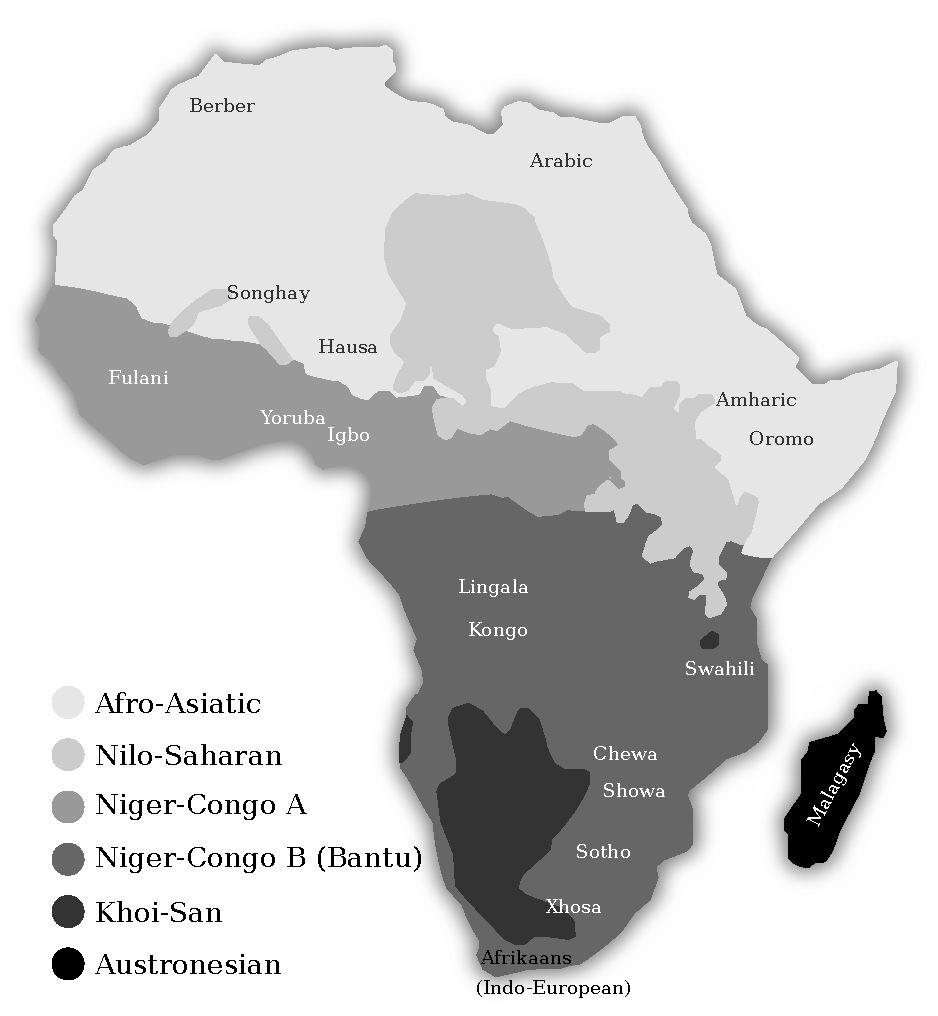
\includegraphics[width=.9\textwidth]{figures/AfricanLanguageFamilies.pdf}
\caption{Language families of Africa\\\tiny Map adapted by Sebastian Nordhoff from \url{https://commons.wikimedia.org/wiki/File:African_language_families_en.svg} (c) Mark Dingemanse (original PNG version); \href{Pmx}{https://fr.wikipedia.org/wiki/Utilisateur:Pmx} (SVG version), CC BY-SA 3.0}
\label{fig:African:1}
\end{figure}
Africa is not only a mineral resource rich continent, it is also a linguistic resource rich continent. Not only are there many languages on the African continent, Africans also exhibit a rich polyglottic repertoire in multilingual societies with many individual Africans, particularly in urban centres, speaking an average of four to five languages per person. Indeed, Africa has the second largest number of languages among the continents. According to \citet{Simons2020}, there are at least 7,102 living languages in the world and 2,138 of them are in Africa.\footnote{We use the term \textit{African languages} (or the \textit{Languages of Africa}) broadly to refer to languages indigenous to the African continent. This term is to be distinguished from the term \textit{Languages in Africa} which would comprise the indigenous languages and non-indigenous languages including former colonial languages like English, French, and Portuguese, which continue to be used as “official” languages in many African countries.} African languages belong to a diverse set of language families, mainly including the Niger–Congo language family (divided into Niger–Congo A and Niger–Congo B, which comprises the Bantu languages), the Afro-Asiatic language family, and the Nilo-Saharan language family, as well as members of the disputed Khoisan language family \citep{Guldemann:Khoisan}; see \figref{fig:African:1}.\footnote{As suggested by one reviewer, Austronesian languages,
  especially on the islands to the East of Africa, like Madagascar,
  ought to also be included in \figref{fig:African:1}; see
  \citetv{chapters/Austronesian} for more on Austronesian
  languages.  In addition, we
  should also acknowledge that not many people believe in the genetic
  unity of “Khoisan” language family anymore.}

The great amount of language diversity on the African
 continent and elsewhere is of interest to linguists and other scholars who believe in the need for linguistic and cultural diversity, and therefore the need to document and preserve these languages and their associated cultures. This diversity itself is a double-edged sword \citep{Bodomo2017}. On the one hand, each of these 2,138 languages in Africa is the basis of a rich culture as languages are the main media through which we express and convey our cultural values. On the other hand, the fact that we have many languages within each of the 55 polities in Africa means that we face serious challenges and problems for language policy formulation and language planning. With this brief mention of the language situation, we now sketch some salient features of African languages in \sectref{sec:African:1.2}.


\subsection{Salient linguistic features of African languages}
\label{sec:African:1.2}

African languages have contributed a lot in informing descriptive and theoretical frameworks for analyzing the world’s languages:

\begin{quote}
In brief, whether the search for universals is pursued along the lines
of cross-linguistic generalizations, as recommended by Comrie,
building on the work of Greenberg and others, or it is conceived of in
terms of the biologically specified abstract principles that determine
the form of human grammars and characterize the content of the
language responsible cognitive structures, it is clear that African
languages will definitely continue to make valuable contributions to
progress in generative grammar.   \citep[202]{Mchombo1997}
\end{quote}

\largerpage
Thirty years ago, in her plenary address \textit{African Languages and Syntactic Theories} on the occasion of the 20th Annual Conference on African Linguistics, Joan Bresnan recognized the impact of African languages on syntactic theories in these aspects: logophoricity, topic/subjecthood, agreement, argument asymmetries, and the syntax of verbs. But the impact was thought to be fairly mild compared to advances in phonology \citep{Bresnan1990}. As time went by, \citet[15]{Henderson2011} asserts that the significant development in this area “has been the exponential increase in syntax researchers who are interested in African languages, along with the sheer volume of work they have produced”. 

The complex morphology of many African languages has been of great interest among linguists, lending support to the study of morphosyntax largely dominated by Bantu languages \citep{bresnan1995the-lexical,Mchombo1980,Mchombo1997,Mchombo:Arg,Mchombo2003,Mchombo2004,Moshi:Locatives,Morimoto:LFG2002,Matambirofa:Causative}. The syntactic derivation of the verb stem in Bantu languages typifies the highly agglutinative nature of these languages, including various suffixes (sometimes called extensions) and prefixes associated with negation, tense/aspect, modality, markers of agreement with the subject and the object, as shown in \REF{ex:African:1}.

\ea\label{ex:African:1} Swahili \citep[152--153]{Petzell2004}\\
\ea\label{ex:African:1a}
\gll si{}-ku-mw-on-a\\
     {\NEG}.\gloss{sm}-{\NEG}.\gloss{t}-\gloss{om}-see-\gloss{fv}   \\
\glt‘I didn’t see him/her.’
\ex\label{ex:African:1b}
\gll  Erik a-li-pig-i-w-a simu na mwalimu.\\
      Eric  \gloss{sm}-{\PST}-ring-{\gloss{appl}}-{\PASS}-\gloss{fv} phone by  teacher\\    
\glt ‘Eric was rung by the teacher.’
\z
\z

Example \REF{ex:African:1a} involves the phenomenon of negation spread in which \textit{si} is both a negative marker and a subject marker. In this case, the morpheme \textit{si} can be called a \textit{portmanteau morph}, i.e., a single morpheme expressing two meanings. Portmanteau morphs and feature spreading such as the negation spread are said to be frequent phenomena in Bantu and other non-Bantu languages such as Mande. In \REF{ex:African:1b}, it is demonstrated that these affixes follow a strict order and certain combinatorial restrictions. For example, the applicative comes before the passive in Swahili.

In general, \citet{CreisselsGood2018} provide a good context to the discussion of African languages with a list of generalizations regarding the state of the art of the morphosyntactic typology of the languages of the continent. These features are listed in \REF{ex:African:2} below \citep[709--710]{CreisselsGood2018}:

\ea\label{ex:African:2}
\ea The ergative type of core syntactic role coding is exceptional among African languages. 
\ex Case-marked subjects or objects are less common among African languages than at world level. 
\ex The so-called “marked-nominative” type of case contrast between subjects and objects is exceptional in other parts of the world but very common among African languages that have a case contrast between subjects and objects. 
\ex Obligatory agreement of transitive verbs with their object does not seem to be attested among African languages. 
\ex Second-position clitics are relatively common in the languages of the world, but exceptional among African languages. 
\ex In a relatively high proportion of African languages, the construction of verbs with an argument frame of the type giver–given–recipient tends to assimilate the recipient (rather than the thing given) to the patient of prototypical transitive verbs, and double object constructions are particularly frequent. 
\ex Focus strategies implying morphosyntactic alternations, and in particular focus marking by means of verbal inflection, are particularly common in Africa. 
\ex The use of special verb forms in sequential constructions is particularly widespread among African languages. 
\ex Applicatives are particularly common in Africa, and a relatively high proportion of African languages make a wide use of obligatory applicatives and of various types of non-canonical applicatives.
\ex Classifier systems are exceptional among African languages. 
\ex Relatively few African languages are devoid of a morphological plural or have a morphological plural restricted to a subset of nouns occupying a high position in the animacy hierarchy. 
\ex African languages that do not use the same morpheme as a noun phrase coordinator and as a comitative adposition are relatively rare. 
\ex The proportion of languages with a syntactically flexible constituent order is much lower among African languages than at world level.
\ex The constituent order SOVX, relatively rare at world level, is relatively frequent among African languages.
\ex Clause-final negative particles occur among African languages much more frequently than in other parts of the world. 
\ex Changes in the constituent order triggered by negation are particularly common among African languages. 
\ex True relative pronouns are particularly rare in African languages, and the use of dependent verb forms in postnominal relatives, relatively rare in the languages of the world, is common among African languages. 
\ex Logophoricity is particularly widespread among African languages. 
\ex Systems of coding of spatial relations in which the distinction location at/movement towards/movement from manifests itself exclusively on verbs are more frequent in Africa than in most other parts of the world.
\z
\z

\largerpage
Admittedly, when it comes to the analyses of African languages in LFG, it is hard not to be “Bantu-centric”, given the pioneering work done by Sam Mchombo and Joan Bresnan. In more recent times, however, much more work is being produced in non-Bantu languages, and we have tried to include the analyses on these non-Bantu languages as much as possible. These mainly include Wolof, Tigrinya, Soso, Wan, Yąg Dii, Malagasy, Dagaare, and Akan. In \sectref{sec:African:2}, we illustrate the analyses of many of these features.

\section{Major African language grammatical phenomena analysed in LFG}
\label{sec:African:2}
\largerpage

In this section, the longest in the chapter, we do a concise analysis of major constructions and grammatical phenomena in African languages from an LFG perspective. We begin with the lexical integrity principle, showing how data from African languages have been used to illustrate one of the best known principles in the LFG theoretical framework. We then move on to discuss argument structure and morphology, agreement, reciprocal marking, locative inversion, serial verbs, and discourse functions.

\subsection{Lexical integrity principle}
\label{sec:African:2.1}

This subsection begins with a constraint on the architecture of grammar inspired by African language structure. When we encounter a sequence of morphemes in African languages, a natural question to ask is: what is indeed a word? In the framework of Lexical Functional Grammar, the lexical integrity principle has been of great importance with respect to c(ategorial)-structure and f(unctional)-structure in clarifyng that the morphemic structure of words differs from the c-structure of phrases both in constituents and principles of combination. In their seminal paper, \citet{bresnan1995the-lexical} elicit a great deal of evidence from Bantu noun class markers in support of the lexical integrity principle. They argued that “the Bantu noun class markers are a particularly fruitful domain for investigations of lexical integrity because they straddle the borderlines between syntax and morphology and between inflection and derivation” (\citealt[183]{bresnan1995the-lexical}).

Bantu noun class markers have a mixed inflectional and derivational nature when they mark nominals for number and gender, specifying the agreement forms of determiners, modifiers and predicates. The number classes, on one hand, trigger the syntactic agreement as an inflectional process, and on the other hand, the gender classes change the semantic class of the stem since they are associated with semantic properties such as animacy, configuration, location, size, plurality or quality and the process is seen as derivational. The standard morphological analysis was strongly advocated by \citet{Doke1929,Doke1935}, in which the class markers are analyzed as morphologically bound morphemes. However, this position has been challenged alternatively by the syntactic analyses (e.g. \citealt{Myers1987}) or the head-movement theories of word derivation (e.g. \citealt{Kinyalolo1991,Carstens1991}). Throwing themselves into this debate, \citet{bresnan1995the-lexical} draw the evidence that supports the lexical integrity principle from the morphology and syntax of Bantu noun class prefixes by applying a couple of effective tests of lexical integrity to the class markers of nouns in Chiche\^wa and other Bantu languages. Four main tests go to build up the argument.

\subsubsection{Test 1: phrasal recursivity}

The central idea of phrasal recursivity is that the arbitrarily deep embedding of syntactic phrasal modifiers is not allowed in word-internal constituents. For Bresnan and Mchombo, there are mixed results on this front due to the so-called alternative concord when modifiers simultaneously show concord with any of several class markers on the same noun \citep[195]{bresnan1995the-lexical}, as shown in example \REF{ex:African:3}. 

\ea\label{ex:African:3} Chishona \citep[104]{Myers1987}\\
    \gll pa-mu-shá uyo p-ósé pa-káchéna\\
        16-3-home  that.3 16-all  16-white\\
    \glt ‘at that whole white house’
    \z

\largerpage[2]
The noun `home' is preceded by two noun class markers from classes 16 and 3. Interestingly, the first following modifier agrees with the inner class 3 marker and the final two agree with the outer class 16 marker. \citet{Myers1987} provides the following syntactic representation:

\ea\label{ex:African:4}\small
\begin{forest}
  [NP,baseline,[N$'$ [N\textsubscript{2}[pa\\class 16]]
            [NP [N$'$ [N\textsubscript{cl} [mu\\class 3]]
                      [NP [N$'$ [N [shá\\home]]]]]
                [Det [uyo\\that.3]]]]
      [Det [pósé\\16-all]]]
\end{forest}
\z
\clearpage
This representational analysis also correctly accounts for the fact that the inner concord modifiers must precede the outer ones as indicated by the ungrammaticality in \REF{ex:African:5}.  

\ea\label{ex:African:5} Chishona\\
\gll *pa-mu-shá apo w-ósé pa-káchéna\\
     16-3-home   that.16  3-all    16-white\\
     \glt \z

The same holds true for Chiche\^wa, shown below in \REF{ex:African:6a}--\REF{ex:African:6d}.

\ea Chiche\^wa\\
\ea\label{ex:African:6a}
    \gll pa  mu-dzi p-áthú p-ônse\\
        16  3-village 16-our 16-all\\
    \glt ‘at all of our village’
\ex
   \gll  pa mu-dzi w-áthú p-ônse\\  
        16  3-village 3-our   16-all\\
   \glt‘at all of our village’
\ex
   \gll  pa mu-dzi w-áthú w-ônse\\
        16  3-village  3-our    3-all\\
   \glt‘at all of our village’
\ex\label{ex:African:6d}
    \gll *pa mu-dzi p-áthú w-ônse\\
    16  3-village 16-our  3-all\\
    \glt
\z
\z

But the syntactic analysis of \citet{Myers1987} does not necessarily apply to all class markers. As a matter of fact, it turns out that the class marker 16 in these examples belongs to the locative classes comprising of 16, 17 and 18, and an alternative concord is only possible with these locative classes. As for the nonlocative class markers, they are prefixed to the nouns and noun stems without the recursive structure of syntactic NPs, where alternative concord is impossible, as shown in (\ref{ex:African:7}).

\ea\label{ex:African:7} Chiche\^wa\\
\ea 
   \gll ka-mu-ndá k-ánga\\
       12-3-field   12-my\\
   \glt ‘my small field’
\ex
   \gll *ka-mu-ndá w-ánga\\
   12-3-field    3-my\\
   \glt
\z
\z

\subsubsection{Test 2: inbound anaphoric islands}

The inbound anaphoric islands test can also tell a true syntactic phrase from a derived word. According to this test, anaphoric and deictic uses of pronouns should occur within the phrasal NP complement to a class marker. Again it is true with the locative class markers but not with the other class markers as shown in \REF{ex:African:8} and \REF{ex:African:9}.

\ea\label{ex:African:8} Chiche\^wa
\ea\label{ex:African:8a}
    \gll mu iyi\\
        18  9.this\\
    \glt ‘in this (e.g. house)’
\ex
    \gll pa icho\\
    16 7.that\\
    \glt ‘on that (e.g. hat)’
\ex\label{ex:African:8c}
    \gll ku ǐwo\\
    17  6.them\\ 
    \glt ‘to them (e.g. pumpkins)’ 
\z
\z

\ea\label{ex:African:9} Chiche\^wa
\ea\label{ex:African:9a}
    \gll *chi iyi\\
        7    9.this\\
    \glt
\ex
    \gll  *ka icho\\
    12   7.it\\
    \glt
\ex\label{ex:African:9c}
    \gll *ti ǐwo\\
    13  6.them\\
    \glt
\z
\z

Since morphological words are inbound anaphoric islands, the ungrammaticality of the examples in \REF{ex:African:9} can only be explained by the morphological analysis of these prefixes instead of the syntactic analysis shown in \REF{ex:African:8}.

\subsubsection{Test 3: conjoinability}

As expected, the locative classes pass the conjoinability test. Following the syntactic analysis, two NP complements should be conjoinable under a single class marker, shown below in \REF{ex:African:10}. However, the other class markers fail the test as shown in \REF{ex:African:11}.
\newpage

\ea\label{ex:African:10} Chiche\^wa
\ea
    \gll Mu-ku-pít-á ku [m-sika kapéná m-zinda]?\\
        II.{\PL}/\gloss{hon}.{\SBJ}-{\PROG}-go-{\IND}    17             3-market or         3-city \\
    \glt ‘Are you going to the market or the city?’
\ex
    \gll A-na-gw-ér-á m [chi-tsȋme kapéná chĭ-gwa]?\\
        1{\SBJ}-{\gloss{rec}.\PST}-fall-{\gloss{appl}}-{\IND}     18    7-well       or           7-valley\\
    \glt ‘Did he fall into the well or the valley?’
\ex
    \gll Mu-na-ík-á pa [m-pando kapéná m-tŏndo]?\\
        II.{\PL}/\gloss{hon}.{\SBJ}-{\gloss{rec}.\PST}-put-{\IND}  16       3-chair      or          3-mortar\\
    \glt ‘Did you put (it) on the chair or the mortar?’
\z
\z

         
\ea\label{ex:African:11} Chiche\^wa
\ea
     \gll  *Mu-na-chéz-á ndí m- [phunzitsi kapéná sangalatsi]?\\
     II.{\PL}/\gloss{hon}.{\SBJ}-{\gloss{rec}.\PST}-converse-{\IND}    with 1- teacher      or         entertainer\\
     \glt ‘Did you converse with the teacher or entertainer?’
\ex
     \gll *A-na-b-á ka- [m-pando kapéná m-tŏndo]?\\
           1{\SBJ}-{\gloss{rec}.\PST}-steal-{\IND} 12   3-chair      or          3-mortar\\
      \glt ‘Did he steal a little chair or a little mortar?’
\z
\z
      
\subsubsection{Test 4: gapping}

Under this test, it is possible to gap the noun following the locative class marker. In contrast, none of the other class markers allow this gapping, as shown in (\ref{ex:African:12}).

\ea\label{ex:African:12} Chiche\^wa
\ea
    \gll  A-nyamǎta a-na-vín-á njerero pa bwaló lá mfúmú Kapanga ndí
    pá (bwaló) lá mfúmú Kapatuka. \\
     2-boy            2{\SBJ}-{\gloss{rec}.\PST}-dance-{\IND}  9.name.of.dance
         16  5.courtyard 5\gloss{asc} 9chief     K.            and  16 5.courtyard
         5\gloss{asc} 9chief     K.   \\
    \glt ‘The boys danced the njerero dance on Chief Kapanga’s  courtyard and on Chief Kapatuka’s (courtyard).’
\ex
    \gll *Kodí áná awa a-ku-fún-á m-pira w-á mphira kapéná m-*(pira)
    w-á nsanza?\\
       Q      2.child   2this  2{\SBJ}-{\PROG}-want-{\IND}  3-ball    3-\gloss{asc}
            9.rubber or          3-(ball)      3-\gloss{asc} 10.rag \\
    \glt ‘Do these children want a rubber ball or a rag ball?’
\z
\z

All these tests show that the locative class markers are syntactically independent and all the others are morphological prefixes. \citet{bresnan1995the-lexical} provided an explanation with regard to the split between the syntactic and morphological class markers. As hypothesized by \citet{Greenberg1977,Greenberg:Gender}, the class markers in Niger-Congo have evolved historically from syntactic elements of NPs into being morphologically bound as prefixes or suffixes. Along this line, it is possible that this process of historical change has been completed for most of the class markers of proto-Bantu that became prefixes, but a few like locatives retained their syntactic behavior as nominal constituents. 

According to \citet{bresnan1995the-lexical}, the fact that agreement is marked both syntactically and morphologically does not violate the lexical integrity principle:

\begin{quote}
By factoring apart the syntactic levels of f-structure and c-structure, we can distinguish naturally between structure-dependent syntactic principles (e.g., constituent order), which respect lexical integrity, and function-depen\-dent syntactic principles (e.g., agreement), which do not. \citep[213]{bresnan1995the-lexical}
\end{quote}

In the LFG framework, the correspondence between structural form and syntactic function is in general imperfect. Take Bantu noun class markers, for example. Here changes in form can occur partly independent of changes in function. As a result, this lends strong support to the lexical integrity principle. With this illustration of the lexical integrity principle, we now go on to discuss argument structure in \sectref{sec:African:2.2}.

\subsection{Argument structure and morphosyntax}
\label{sec:African:2.2}

In this subsection we discuss two main constructions, applicatives and objective asymmetries mainly in Bantu languages, before outlining some recent works in mainly non-Bantu languages.

\largerpage[-1]
\subsubsection{Applicative constructions}


The discussion of grammatical functions came to the fore in the 1980s and early 1990s \citep{Marantz1984,Baker1988,Alsina1992,AlsinaMchombo1990,AlsinaMchombo:Appl,BresMosh90}. Valency-changing operations like the passive, applicative, causative and similar alternations had raised the question whether grammatical functions (GF) should be seen to be primitives or derivatives. Bantu languages contributed a lot to this discussion since these languages are characterized by applicative, causative and passive morphemes (see \REF{ex:African:1b} for example). 

This section centers on a critique made by \citet{AlsinaMchombo1990} on \citet{Baker:Theta} over applicatives in Chiche\^wa. \citet{Baker:Theta} proposes an asymmetry in the assignment of the beneficiary and instrumental theta-roles. For Baker, instrumentals are assigned their theta-roles as NP sisters of the verb, while beneficiaries are theta-marked in a PP complement to the verb. In other words, beneficiaries get their theta-role indirectly from the verb through the PP but instrumentals are theta-marked directly by the verb. According to Alsina and Mchombo, Baker’s theory is particularly successful in two aspects \citep[495]{AlsinaMchombo1990}:

\begin{exe}\label{ex:African:13}
\ex \begin{xlist}
\ex Word order: while the beneficiary NP must precede a theme/patient NP in the verb phrase, the instrumental NP may either precede or follow it.
\ex Object markers: while only the applied object in a beneficiary
applicative may be expressed by means of an object marker, either the
applied or the patient/theme object in an instrumental applicative may
be so expressed.
\end{xlist}
\end{exe}


\largerpage[-1]
At the same time, they also adduced three types of evidence against Baker’s theta theoretic asymmetry.

\subsubsubsection{Extraction facts}

As observed by \citet{Baker:Theta}, a patient or a theme can be extracted both in beneficiary \REF{ex:African:14a} and in instrumental applicatives \REF{ex:African:15a}, but in contrast, it is not possible to extract a beneficiary object \REF{ex:African:14b} as an instrumental \REF{ex:African:15b}.

\ea\label{ex:African:14} Chiche\^wa
\ea\label{ex:African:14a}
    \gll Īyi ndi mphátso iméné chítsîru chí-ná-gúl-ír-a atsík\=ana.\\
        9.this be   9.gift      9.{\REL} 7.fool    7{\SBJ}-{\PST}-buy-{\gloss{appl}}-\gloss{fv}
          2.girls\\
    \glt ‘This is the gift that the fool bought for the girls.’
\ex\label{ex:African:14b}
    \gll *Āwa  ndi atsíkána améné chítsîru chí-ná-gúl-ír-a mph\^atso.\\
       ~~2.these be  2.girls    2.{\REL} 7.fool   7{\SBJ}-{\PST}-buy-{\gloss{appl}}-\gloss{fv} 9.gift \\
    \glt ‘These are the girls that the fool bought the gift for.’
\z
\z

\newpage
\ea\label{ex:African:15} Chiche\^wa
\ea\label{ex:African:15a}
    \gll Īli ndi dengu liméné ány\v{a}ni       á-kú-phwány-ír-a mw\v{a}la.\\
        5.this be  5.basket 5.{\REL} 2.baboons 2{\SBJ}-{\PROG}-break-{\gloss{appl}}-\gloss{fv}        3.stone\\
    \glt ‘This is the basket that the baboons are breaking with a stone.’
\ex\label{ex:African:15b}
    \gll \={U}wu   ndi  mwalá úméné ány\v{a}ni
      á-kú-phwány-ír-a dēngu.\\
       3.this  be  3.stone 3.{\REL} 2.baboons 2{\SBJ}-{\PROG}-break-{\gloss{appl}}-\gloss{fv} 5.basket \\
    \glt ‘This is the stone that the baboons are breaking the basket with.’
    \z
    \z

\citet{Baker:Theta} explains these differences on the basis of the \textit{nonoblique-trace filter}. Unfortunately, the whole analysis collapses given the fact that there are grammatical instances of extractions of beneficiaries or goals in a Chiche\^wa passive sentence \citep[498]{AlsinaMchombo1990}:

\ea\label{ex:African:16} Chiche\^wa\\
    \gll \={A}wa      ndi  atsíkána  améné  á-ná-gúl-ír-ídw-á mph\^{a}tso.\\
        2.these  be   2.girls     2.{\REL}  2{\SBJ}-{\PST}-buy-{\gloss{appl}}-{\PASS}-\gloss{fv} 9.gift\\
    \glt ‘These are the girls that were bought a gift.’
    \z

\subsubsubsection{Transitivity effects}

Baker’s proposed D-structure distinction between beneficiaries and instrumentals predicates that beneficiary applicatives cannot be formed from intransitive verbs. However, \citet{AlsinaMchombo1990} prove it to be incorrect again, as in \REF{ex:African:17}.

\ea\label{ex:African:17} Chiche\^wa\\
    \gll Y\^{e}su       a-ná-wá-f-er-a                       (anthu).\\
        1.Jesus  1{\SBJ}-{\PST}-2{\OBJ}-die-{\gloss{appl}}-\gloss{fv}  \phantom{(}2.people\\
    \glt ‘Jesus died for them (the people).’
    \z

\subsubsubsection{Locative applicatives}

According to \citet[503]{AlsinaMchombo1990}, “locative applicatives constitute a crucial source of evidence for evaluating \citegen{Baker:Theta} theory”. In Baker’s theory, beneficiaries and locatives are conceptually similar because they are both theta-marked by the verb via a preposition. In contrast, the facts show that locatives behave like instrumentals and not like beneficiaries considering things like word order, object marking, and relativization.

Consequently, a classical transformational approach appears to be quite problematic when dealing with applicatives in Chiche\^wa given its complex morpho\-syntax.

\subsubsection{Object symmetries/asymmetries}


So far, we have briefly discussed one asymmetrical object type:
applicatives. This subsection will look deeper into this construction
in parallel to the symmetrical type. The distinction between the two
types is associated with \textit{primary object} syntactic properties
of passivizability, object agreement, adjacency to the verb, and the
like. The asymmetrical object type language means that only one of the
postverbal NPs exhibits \textit{primary object} syntactic properties,
while in the symmetrical object type language there are more than one
NPs that can do so.\footnote{The asymmetrical type includes languages
such as Kiswahili, Chimwi:ni, Hibena and Chiche\^wa, while the
symmetrical type includes languages such as Kinyarwanda, Kihaya,
Kimeru, Mashi, and Luyia (or Luhya).} \citet[149--157]{BresMosh90}
identify the typological differences based on their observation on
Kichaga (symmetrical) and Chiche\^wa (asymmetrical).\footnote{The examples in this chapter are selected from
various papers covering a wide range of African languages. We cannot
guarantee their consistency in orthography. All we can do is
transcribe them as originally as possible. In terms of tones, the
symbol \H{}  represents a superhigh tone, \'{} a high tone, ˇa rising
tone,\^{}  a falling tone,\`{} a low tone, and ˉ a superlow tone.}

\ea\label{ex:African:18} Kichaga
\ea\label{ex:African:18a}
    {\gll N-\H{a}-\H{i}-lyì-í-à  \`{m}-kà    k-élyà.\\
        {\FOC}-1{\SBJ}-{\PROG}-eat-{\gloss{appl}}-\gloss{fv} 1-wife  7-food\\}\jambox*{V NP\textit{\textsubscript{ben}}  NP\textit{\textsubscript{pt}}}
    \glt ‘He is eating food for/on his wife.’
\ex\label{ex:African:18b}
    {\gll \`{M}-kà   n-\H{a}-\H{i}-lyì-í-ò k-élyâ.\\
        1-wife 1{\SBJ}-{\PROG}-eat-{\gloss{appl}}-{\PASS}  7-food\\}  \jambox*{NP\textit{\textsubscript{ben}} V\textsubscript{pas} NP\textit{\textsubscript{pt}}}
    \glt ‘The wife is being benefited/adversely affected by someone eating the food.’
\ex\label{ex:African:18c}
    {\gll K-èlyá k-\H{i}-lyì-í-ò \`{m}-kà.\\ 
        7-food    7{\SBJ}-{\PROG}-eat-{\gloss{appl}}-{\PASS} 1-wife\\} \jambox*{NP\textit{\textsubscript{pt}} V\textsubscript{pas} NP\textit{\textsubscript{ben}}}
    \glt ‘The food is being eaten for/on the wife.’
\z
\z
    

The Kichaga examples \REF{ex:African:18b}--\REF{ex:African:18c} show that any object in the symmetrical type can be passivized, but in Chiche\^wa, examples like \REF{ex:African:18c} are ungrammatical \citep{Baker:Theta}.

Another difference is related to object markers, illustrated in \REF{ex:African:19}.

\ea\label{ex:African:19} Kichaga
\ea\label{ex:African:19a}
    \gll N-\H{a}-\H{i}-\`{m}-lyì-í-à k-èlyâ. \\
        {\FOC}-1{\SBJ}-\PROG-1{\OBJ}-eat-{\gloss{appl}}-\gloss{fv}  7-food \\\jambox*{OM\textit{\textsubscript{ben}}-V\textsubscript{stem}  NP\textit{\textsubscript{pt}}}
    \glt ‘He/She is eating food for/on him/her.’
\ex\label{ex:African:19b}
    {\gll N-\H{a}-\H{i}-kì-lyí-í-à    \`{m}-kà.\\ 
       {\FOC}-1{\SBJ}-\PROG-7{\OBJ}-eat-{\gloss{appl}}-\gloss{fv}  1-wife \\}\jambox*{OM\textit{\textsubscript{pt}}-V\textsubscript{stem}  NP\textit{\textsubscript{ben}}}
    \glt ‘He/She is eating it for/on the wife.’
\ex\label{ex:African:19c}
    {\gll N-\H{a}-\H{i}-kì-ḿ-lyì-\H{i}-à.\\ 
        {\FOC}-1{\SBJ}-\PROG-7{\OBJ}-1{\OBJ}-eat-{\gloss{appl}}-\gloss{fv}\\}\jambox*{OM\textit{\textsubscript{pt}}-OM\textit{\textsubscript{ben}}-V\textsubscript{stem}}
    \glt ‘He/She is eating it for/on him/her.’
\z
\z

In Kichaga, the object marker can be put on the verb from any or all of the multiple objects. Again, cases such as \REF{ex:African:19b} and \REF{ex:African:19c} are not allowed in Chiche\^wa.

\citet{BresMosh90} also compared the two types in terms of unspecified
object deletion, reciprocalization and interactions of object
properties. They went on to discuss the problems posed by the data for
previous theories \citep{Gary:UG,perlmutter1983some,Marantz1984,Baker:Theta,Kiparsky1988}. Along the lines of
\citet{AlsinaMchombo:ApplDraft}, \citet{bresnan1989locative} and
\citet{Alsina1999}, \citet{BresMosh90} show that the LFG treatment is
capable of providing a single parameter of variation for the
symmetrical and asymmetrical object types from which all the
typological differences follow, instead of postulating multiple
unrelated differences in the grammar of the two types of languages. In
doing so, they decomposed syntactic functions by two crucial
properties: [$-r$] and [$+o$], schematized in
\REF{ex:African:20}.

\ea\label{ex:African:20}
\begin{tabular}[t]{ll@{\hspace*{4em}}ll}
  $\left[\begin{array}{c}-{r}\\-{o}\end{array}\right]$ & \SUBJ &
  $\left[\begin{array}{c}+{r}\\-{o}\end{array}\right]$ & \OBLTHETA\\[4ex]
  $\left[\begin{array}{c}-{r}\\+{o}\end{array}\right]$ & \OBJ &
  $\left[\begin{array}{c}+{r}\\+{o}\end{array}\right]$ & \OBJTHETA
\end{tabular}
\z

However, there is a peculiarity in applicative and dative constructions. Following \citet{AlsinaMchombo:ApplDraft}, Bresnan and Moshi acknowledged that there is a limitation concerning the applied beneficiary and recipient roles, i.e., they universally lack the [$+o$] classification and receive the [$-r$] classification. An asymmetrical object parameter was therefore proposed:

\ea\label{ex:African:21} Asymmetrical Object Parameter (AOP)\\[1ex]
\begin{tabular}{cccc}
  * & $\theta$ & ... & $\theta$\\
    & \textbar && \textbar\\
    & [$-r$] & & [$-r$]
\end{tabular}
\z

For ditransitive constructions in Chiche\^wa \citep{MchomboFirmino1999}, the applied NP must be adjacent to the verb if it is a beneficiary or recipient; otherwise, either the patient NP or the applied NP may be adjacent to the verb \citep[172]{BresMosh90}. Serving as the parameter of variation, it states that only one role can be intrinsically classified as unrestricted. The idea is illustrated in \REF{ex:African:22}.

\ea\label{ex:African:22}
\begin{tabular}[t]{lccccc}
  & `eat-for{\textlangle} & \textit{ag} & \textit{ben\textsubscript{appl}} & \textit{pt} & {\textrangle}'\\[1ex]
  AOP:  && [$-o$] & [$-r$] & [$+o$]\\
  defaults: && [$-r$] & & [$+r$]\\
  \cline{3-5}
  & & \SUBJ & \SUBJ/\OBJ & \OBJTHETA\\
  well-formedness: & & \SUBJ & \OBJ & \OBJTHETA\\
\end{tabular}
\z

Based on \citegen{AlsinaMchombo:ApplDraft} extended version of intrinsic classifications to account for applicative and dative constructions, the applied beneficiary or recipient role (traditionally called \textit{indirect objects}) can only be [$-r$], whereas the patient can be either [$-r$] or [$+o$]. Similarly in Kichaga, the applied beneficiary role will always be [$-r$], however, since the AOP does not apply to the symmetrical type, the patient can be either [$-r$] or [$+o$] as shown in \REF{ex:African:23} and \REF{ex:African:24}. The only problem with \REF{ex:African:23} is that two unrestricted roles will lead to a violation of the final well-formedness condition of Function-Argument Biuniqueness which states that each expressed lexical role must be associated with a unique function, and conversely. So the patient role can only take the [$+o$] option in the active as shown in \REF{ex:African:24}.

\ea\label{ex:African:23}
\begin{tabular}[t]{lccccc}
  & `eat-for{\textlangle} & \textit{ag} & \textit{ben\textsubscript{appl}} & \textit{pt} & {\textrangle}'\\[1ex]
            && [$-o$] & [$-r$] & [$+o$]\\
  defaults: && [$-r$]\\
  \cline{3-5}
  & & \SUBJ & \SUBJ/\OBJ & \SUBJ/\OBJ\\
  well-formedness: & & \SUBJ & \OBJ & *\\
\end{tabular}
\z

\ea\label{ex:African:24}
\begin{tabular}[t]{lccccc}
  & `eat-for{\textlangle} & \textit{ag} & \textit{ben\textsubscript{appl}} & \textit{pt} & {\textrangle}'\\[1ex]
            && [$-o$] & [$-r$] & [$-o$]\\
  defaults: && [$-r$] & & [$+r$]\\
  \cline{3-5}
  & & \SUBJ & \SUBJ/\OBJ & \OBJTHETA\\
  well-formedness: & & \SUBJ & \OBJ & \OBJTHETA\\
\end{tabular}
\z

The analysis also explains adequately why in Chiche\^wa only the object that is adjacent to the verb in the active can become the subject in the passive, as seen in \REF{ex:African:25}, while in Kichaga, either object can be passivized, because when one of the two [$-r$] roles is realized as the subject in the passive construction, the other may be the unrestricted object, as shown in \REF{ex:African:26}.

\ea\label{ex:African:25}
\begin{tabular}[t]{lccccc}
  & `eat-for{\textlangle} & \textit{ag} & \textit{ben\textsubscript{appl}} & \textit{pt} & {\textrangle}'\\[1ex]
  AOP:      && [$-o$] & [$-r$] & [$+o$]\\
  Passive : && $\emptyset$\\
  defaults: &&  & & [$+r$]\\
  \cline{3-5}
  & &  & \SUBJ/\OBJ & \OBJTHETA\\
  well-formedness: & & & \SUBJ & \OBJTHETA\\
\end{tabular}
\z

\ea\label{ex:African:26}
\begin{tabular}[t]{lccccc}
  & `eat-for{\textlangle} & \textit{ag} & \textit{ben\textsubscript{appl}} & \textit{pt} & {\textrangle}'\\[1ex]
            && [$-o$] & [$-r$] & [$-r$]\\
  Passive : && $\emptyset$\\
  defaults: &&\\
  \cline{3-5}
  & & & \SUBJ/\OBJ & \SUBJ/\OBJ\\
  well-formedness: & & & \SUBJ & \OBJ & or\\
   & & & \OBJ & \SUBJ\\
\end{tabular}
\z

The single parameter of variation under LFG provides good explanations for other typological differences equally well, namely object deletion, reciprocalization and interactions of object properties, which have been observed between the symmetrical and asymmetrical object types. 

In the LFG literature, two recent works on Setswana are from \citet{Berg:Setswana} and \citet{PretoriusBerg:Aux}. The latter proposes an LFG-based analysis of the tense and aspect features of Setswana auxiliary verbs. In Setswana, auxiliary verbs indicating tense, aspect and time may appear juxtaposed inside a VP, following a specific order determined by the semantic values associated with the auxiliaries. Here we focus on \citet{Berg:Setswana} which analyses Setswana constructions with double objects and double object agreement morphemes. 

\ea\label{ex:African:27} Setswana\\
    \gll Mosadi o-\textbf{di}-rek-el-a mosetsana.\\
     1.woman     1-8-buy-{\gloss{appl}}-\gloss{fv}     1.girl   \\
    \glt ‘The woman buys the girl it’.
    \z

\ea
\begin{tabular}[t]{@{}cc}
  c-structure: & f-structure:\\[1ex]
{\begin{forest}
  [S [NP [N [mosadi]]]
    [VP [V,baseline,[odirekela]]
      [NP [N [mosetsana]]]]]
\end{forest}} & 
{\avm[style=fstr]{[pred & `rek\arglist{subj,\OBJTHETA,obj}'\\
  subj & [pred & `sadi'\\
    nounclass & 1]\\
  \OBJTHETA & [pred & `setsana'\\
    nounclass & 1]\\
  obj & [pred & `pro'\\
    nounclass & 8 ]\\
  ap & +\\
  class & 1\\
  tense & pres\\
  verbtype & main]}}
\end{tabular}
\z

In the end, these works also provide a computational model of these phenomena using the XLE grammar development platform.\footnote{For those who are interested in XLE implementations, they can see them both in \citet{Dione2013} and \citet{Berg:Setswana}.} Other LFG work on argument structure and grammatical functions can be seen in \citet{Zaenen:Kikuyu}, \citet{Mchombo1980,Mchombo1999,Mchombo:Arg,Mchombo2003,Mchombo2004}, \citet{Harford1993}, and \citet{Kioko1995}. For recent papers on this topic within Bantu languages, one may refer to \citet{Matambirofa2010} and \citet{Matambirofa:Causative}.               

\subsubsection{Recent work in argument structure on non-Bantu languages}


As is well known, at least among LFG practitioners, LFG research on African languages has been pioneered and dominated by analyses of Bantu languages, as shown in the previous analyses. In this subsection, we bring to light a few recent studies involving four languages outside the Bantu group: Tigrinya, Wolof, Soso, and Wan, the latter two of which belong to the Mande language family.\footnote{Our special thanks go to one of the reviewers who summarized for us some parts of works included in this section.} Particularly, the discussion of object properties is found in all four languages.

\subsubsubsection{Work on Tigrinya} 

In previous discussions, we have seen that the correlation of properties such as pronominal marking and passive typology has been used in object asymmetries as a proof for primary objecthood (\citealt{BresMosh90}, \citealt{AlsinaMchombo:Appl}, \citealt{Alsina:Passive}). \citegen{Kifle07} analysis reveals that Tigrinya exhibits symmetric properties of objects in its ditransitive constructions, and asymmetric properties in its applicative constructions. 

\ea\label{ex:African:29} Tigrinya
\ea\label{ex:African:29a}
    \gll ʔɨt-omɨ tämäharo n-ät-i mäṣɨḥafɨ-ti tä-wahib-om-wo.\\
     {\DEF}-3{\M.\PL} student.{\PL}  {\OBJ}-{\DEF}-3{\M.\SG}   book.{\PL} {\PASS}-{\PRF}.give-\gloss{sm}.3{\M.\PL}-\gloss{om\textsubscript{1}}.3{\M.\SG}  \\
    \glt ‘The students are given books.’
\ex\label{ex:African:29b}
    \gll ʔɨt-i mäṣɨḥafɨ-ti nɨ-tämäharo tä-wahib-u-womɨ.\\
      {\DEF}-3{\M.\SG} book.{\PL}      {\OBL}-student.{\PL}  {\PASS}-{\PRF}.give-\gloss{sm}.3{\M.\SG}-\gloss{om\textsubscript{1}}.3{\M.\PL}  \\
    \glt ‘The books are given to students.’
\z
\z

The recipient \REF{ex:African:29a} and the theme \REF{ex:African:29b} display primary object properties in the sense that both of them function as subjects in passivization. However, it is observed that only the theme role can function as a subject in passivization when it comes to applicative constructions, as shown in \REF{ex:African:30}. The type of asymmetry found in Tigrinya seems to be the reverse version of the asymmetry found in Bantu languages like Chiche\^wa.

\ea\label{ex:African:30} Tigrinya
\ea\label{ex:African:30a}
    \gll  ʔɨt-i mäṣɨḥafɨ n-saba tä-gäzi-u-la.\\
      {\DEF}-3{\M.\SG} book.{\SG}   \OBL-Saba.{\F}    {\PASS}-{\PRF}.buy-\gloss{sm}.3{\M.\SG}-\gloss{om\textsubscript{2}}.3{\F.\SG}  \\
    \glt ‘The book was bought (for) Saba.’
\ex\label{ex:African:30b}
     \gll *saba mäṣɨḥafɨ tä-gäzi-ʔa\\
     Saba.F book.{\SG}   {\PASS}-{\PRF}.buy-\gloss{sm}.3{\F.\SG}\\
\z
\z

Therefore, in Tigrinya ditransitive clauses, the symmetric objects possess the [$-r$] features classified as \OBJ{s}, while the applied object in an applicative construction functions as \OBJTHETA\ with the [$+r$] feature and  the verbal object is \OBJ\ with the [$-r$] feature. Given these facts, the Tigrinya data pose a particular challenge to the claim made about the correlation between the passive typology and the restrictions on pronominal marking. When applied to Tigrinya \citep{Kifle11}, the grammatical tests commonly used to distinguish between symmetrical and asymmetrical objects do not converge into a single primary object property. In Tigrinya, the applied object often displays the opposite properties to what is predicted by the lexical mapping theory (LMT). 

\subsubsubsection{Work on Wolof} 

In relatively recent research, diverse phenomena in the morphosyntax of Wolof have been analyzed in LFG, including its cleft constructions and their relations to copular constructions \citep{Dione12}, the interaction between Wolof clitics and different grammar components \citep{dione2013handling}, and pro-drop and control constructions \citep{Dione19Clause}. In addition, there are several recent works on Wolof that take a computational approach to handle various aspects of the language within the LFG framework \citep{Dione:Disambiguation,Dione:Pruning,Dione:Finite,Dione2020}.

Among his extensive work on Wolof, \citet{Dione2013} proposes an LFG-based analysis to deal with applicative-causative polysemy in Wolof using a predicate composition approach of complex predicate formation. He postulated an a-structure for each derivation (applicative and causative) by analyzing polysemous suffixes as carrying their own PRED(ICATE) argument structure which they share with other suffixes of the same derivation type. The focus of his work is on Wolof applicative and causative suffixes.

\ea\label{ex:African:31} Wolof
\ea\label{ex:African:31a}
    \gll  Móodu la Faatu wax-al.\\
       Móodu {\FOC}.3{\SG} Faatu  talk-{\gloss{appl}}\\
    \glt ‘Faatu talked to MÓODU.’
    \ex\label{ex:African:31b}
    \begin{tabular}[t]{lc@{}c@{}c@{}c@{}c}
      && \textit{Faatu} && \textit{Móodu}\\
\textit{-al} comitative:  && \SUBJ && \OBJ\\
      && \textbar && \textbar\\
      &`ap{\textlangle}`wax{\textlangle}&\textunderscore&{\textrangle}', &\textsc{arg}&{\textrangle}'\\
      && agt && com
    \end{tabular}
\z
\z

\ea\label{ex:African:32} Wolof
\ea\label{ex:African:32a}
    \gll   Faatu daw-al woto bi.\\
       Faatu   run-{\CAUS}  car   the\\
    \glt ‘Faatu made the car run.’
    \ex\label{ex:African:32b}
    \begin{tabular}[t]{lc@{}c@{}c@{}c@{}c}
      && \textit{Faatu} && \textit{woto}\\
\textit{-al} causative:      && \SUBJ && \OBJ\\
      && \textbar && \textbar\\
      &`caus{\textlangle}&\textsc{arg}, &`daw{\textlangle}&\textunderscore&{\textrangle}'{\textrangle}'\\
      && causer && causee
    \end{tabular}
\z
\z

\hspace*{-1.4pt}Dione proposed a special argument \textsc{arg} as the matrix argument for each derivation type. In the applicative clause \REF{ex:African:31b}, he assumed that \textsc{arg} bears the matrix’s second argument and is underspecified for a comitative, while in the causative clause \REF{ex:African:32b}, \textsc{arg} occupies the subject position and bears the matrix first argument.

\subsubsubsection{Work on Mande}

\citet{Nikitina2011,Nikitina2019} examine a highly unusual basic word order pattern in Mande languages: the rigid S-O-V-X word order, meaning subjects and objects precede the verb, while all oblique arguments and adjuncts follow the verb. For example, 

\ea\label{ex:African:33} Soso, Central Mande\\
\glll  S     O          V               [PP     ~ ~ ]\\
         ń nìngéé fíí-mà ~ í má\\
        1{\SG} cow      give-FUT   2{\SG}  to\\
    \glt ‘I will give you a cow.’
    \z

Mande languages are not regarded as “real” verb-final languages in the sense that arguments of a verb are not realized within the same verb phrase: object noun phrases must be placed next to their verb, but postpositional arguments appear in the position outside the verb phrase. 

\ea\label{ex:African:34}Wan, Southeastern Mande
\ea\label{ex:African:34a}
    \gll  è [kúnà]\textsubscript{VP}  ságlā [yrɛ é gó]\textsubscript{PP}\\
        3{\SG}     \phantom{[}climb      started    \phantom{[}tree  {\DEF} in  \\
    \glt ‘She began to climb onto the tree.’
\ex\label{ex:African:34b}
    \gll  *è kúnà [yrɛ é gó]\textsubscript{PP}  ságlā\\
        3{\SG}   climb    \phantom{[}tree   {\DEF} in        started \\
\ex\label{ex:African:34c}
    \gll  *è [yrɛ é gó]\textsubscript{PP}  kúnà ságlā\\
        3{\SG}   \phantom{[}tree  {\DEF} in       climb   started    \\
\z
\z

Because the oblique argument \textit{yrɛ é gó} does not form a syntactic constituent with the verb \textit{kúnà} that selects for it, it cannot appear next to that verb as shown in \REF{ex:African:34b} and \REF{ex:African:34c}, and only \REF{ex:African:34a} is grammatical in which the verb \textit{kúnà} is embedded in the non-finite complement of the finite verb \textit{ságlā}. \citet{Nikitina2019} explains this unexpected placement of postpositional arguments in terms of a surface-oriented account of high attachment of PPs. 

\ea\label{ex:African:35}Wan, Southeastern Mande\\
    \gll  \`e  á    bɛ̰n\`{\i}   lé      sóg\`{o}-m\`{u}-\`{e} lé\\
        3{\SG} {\PROG}  fear   {\PROG} horse-{\PL}-{\DEF} at \\
    \glt ‘She fears horses.’
    \z

The phrase structure rule in \REF{ex:African:36} allows for PPs to adjoin to the clause \citep{Nikitina2008,Nikitina:Mixing}:

\ea\label{ex:African:36}
\phraserule{IP}{\rulenode{IP\\\UP=\DOWN} \rulenode{PP\\(\UP\ \GF* \OBL)=\DOWN}}
\z

The Kleene star indicates that the PP can contribute information regarding an oblique argument at any level of embedding, but the ambiguity at the c-structure can be solved at the f-structure where the PP is associated with the main verb to satisfy the well-formedness conditions on f-structure. The resulting structures of \REF{ex:African:35} is thus represented below:

\ea\label{ex:African:37}
\begin{tabular}[t]{cc}
c-structure: & f-structure:\\[1ex]
{\begin{forest}
    [IP [{IP\\\UP=\DOWN} [{NP\\(\UP\SUBJ)=\DOWN},baseline,[{\`e\\she},roof]]
        [{I$'$\\\UP=\DOWN} [{á bɛ̰n\`{\i} lé\\is afraid},roof]]]
        [{PP\\(\UP\OBL)=\DOWN} [{sóg\`{o}-m\`{u}-\`{e} lé\\of the horses},roof]]]
\end{forest}} & 
{\avm[style=fstr]{
    [pred & `fear\arglist{subj,obj}\\
      asp & prog\\
      tense & pres\\
      subj & [pred & `pro'\\
        pers & 3\\
        num & sg]\\
      obl & [pred & `horse'\\
        num & pl\\
        def & +\\
        form & le]]}}
\end{tabular}
\z

\subsection{Agreement}
\label{sec:African:2.3}

African languages exhibit an interesting nature of agreement (\citealt{BM87}, \citealt{Culy:FulaPronouns}, \citealt{Mchombo2004}, \citealt{Nsoh2011}). This section will focus on pronouns in particular. Two particular LFG papers dealing with pronouns and agreement are \citet{BM87} and \citet{Dalrymple2015}.

Like other Bantu languages, the subject marker (\gloss{sm}) and object marker (\gloss{om}) in Chiche\^wa indicate agreement in their verbal morphology. For Bresnan and Mchombo, the \gloss{om} is always an incorporated pronoun but the subject NP has two possibilities: a true subject grammatically agreeing with the verb or a topic NP anaphorically agreeing with the subject pronominal in the verb, as shown in \REF{ex:African:38}.

\ea\label{ex:African:38}
\begin{tabular}[t]{cc}
c-structure: & f-structure:\\[1ex]
{\begin{forest} 
    [S [{NP\\(\UP\SUBJ)=\DOWN}]
      [{VP\\\UP=\DOWN} [{V\\(\UP\SUBJ)=\DOWN\\(\UP\PERS)=3\\(\UP\GEND)=x\\(\UP\PRED)=`L\arglist{(\UP\SUBJ)}'},baseline]]]
\end{forest}} &       
\mbox{\avm[style=fstr]{
    [subj & \rnode{subj}{[pers & 3\\
        num & sg\\
        gend & x]}\\
      pred & `L\arglist{\rnode{arg}{\textunderscore}}']}
\CURVE[.3]{-2pt}{0}{subj}{0pt}{270}{arg}}\\[1ex]
c-structure: & f-structure:\\[1ex]
{\begin{forest}
    [S [{NP\\(\UP\TOPIC)=\DOWN}]
      [{VP\\\UP=\DOWN} [{V\\(\UP\SUBJ)=\DOWN\\(\UP\PRED)=\textsc{`pro'}\\(\UP\PERS)=3\\(\UP\GEND)=x\\(\UP\PRED)=`L\arglist{(\UP\SUBJ)}'},baseline]]]
\end{forest}} &       
\mbox{\avm[style=fstr]{
    [topic & \rnode{topic}{[...]}\\
      subj & \rnode{subj2}{[pers & 3\\
        num & sg\\
        gend & x]}\\
      pred & `L\arglist{\rnode{arg2}{\textunderscore}}']}
\DOTCURVE[.3]{-2pt}{0}{subj2}{0pt}{0}{topic}\CURVE[.3]{-1.5pt}{0}{subj2}{0pt}{270}{arg2}}
\end{tabular}
\z

In a recent paper, \citet{Dalrymple2015} carries out a thorough investigation on the complicated pronominal system in Yąg Dii. According to her, Yąg Dii provides counter-evidence to the general assumption that languages do not have grammatical dependencies that are exclusively nonlocal. The following observations are made regarding the distribution of four types of Yąg Dii pronouns \citep[1113]{Dalrymple2015}:

\begin{exe}\label{ex:African:39} 
\ex \begin{xlist}
\ex MÍ: can bear any grammatical function, except for subject of \`{Ą}\`{N} clause; antilogophoric in BI domain 
\ex \`{Ą}\`{N} : must appear as subject of \`{Ą}\`{N}  clause; antilogophoric in BI domain 
\ex BI: appears only in BI domain; can bear any grammatical function (except for some subordinate subject positions within BI domain); coreferent with logophoric antecedent 
\ex ÌI: appears only as subordinate subject within logophoric domain; coreferent with logophoric antecedent
\end{xlist}
\end{exe}

Take the BI pronouns, for example \citep[118]{Bohnhoff1986}:

\ea\label{ex:African:40} Yąg Dii\\
    \gll Nà’á Ø ’ǫd bà’á [Múúsà bà Ø ’ǫ [bà bi\`{n} h\'{\k{i}}\'{\k{i}} lààlɨ  kaalɨ]]. \\
        Mother$_i$ (she$_i$) tells Father \phantom{[}Moses$_j$ \phantom{[}that (he$_j$) says \phantom{[}that he.BI$_{j,*i}$  
        wants to.go town.to \\
    \glt ‘Mother$_i$ tells Father that Moses$_j$ says that *she$_i$/he$_j$ wants to go to town.’
\z

\ea\label{ex:African:41} Yąg Dii\\
    \gll *Nà’á Ø ’ǫd bà’á [bà mí ’ǫ [bà bi\`{n}  h\'{\k{i}}\'{\k{i}} lààlɨ kaalɨ]].\\
      Mother$_i$ (she$_i$) tells Father  \phantom{[}that   I      say \phantom{[}that she.BI$_i$ wants to.go town.to \\
    \glt ‘Mother$_i$ tells Father that I say that she$_i$ wants to go to town.’
\z

The analysis is built on LFG’s binding theory, which is schematized in \REF{ex:African:42} \citep[1114]{Dalrymple2015}.

\ea\label{ex:African:42}
\textsc{\begin{tabular}[t]{cp{4em}p{6em}cp{6em}c}
  (\UPS\ \textsc{ant}) = ((& gf* & gf\textsubscript{pro}& \UP) &gf\textsubscript{ant} &)$_\sigma$\\
  & delimits binding domain & grammatical function of pronoun & & grammatical function of antecedent
\end{tabular}}\\
f-structure:  \avm[style=fstr]{[gf\textsubscript{ant} & [antecedent]\\
    ...gf*...gf\textsubscript{pro} & [pronoun]]}
\z

The equation dictates that the antecedent must be found within the binding domain \textsc{(gf*~gf\textsubscript{pro}~\UP)}. In order to constrain the distribution of the four types of pronouns, \citet{Dalrymple2015} adds the \textsc{log} feature to the inventory of features that are universally available in the binding domain, inspired by \citet{bresnan2001lexical}, \citet{Adesola2006}, \citet{Asudeh2009}, and \citet{Strahan:LFG09,Strahan2011}. 

The binding constraints for BI was proposed by Dalrymple as follows:

\ea\label{ex:African:43}
\textsc{(\UPS\ antecedent) =
  ((\begin{tabular}[t]{@{}cccc@{}c}gf\textsubscript{log} & gf* & \UP)& subj &)$_\sigma$\\
    ($\rightarrow$ log) & $\neg$($\rightarrow$ log) \\
1 & 2 & & 3
\end{tabular}}
\z

The logophoric pronoun must appear within the logophoric domain which is the f-structure value of the \textsc{gf\textsubscript{log}} feature. The numbers occur under each element of binding equation where constraints are imposed. For example, the number 2 states that the BI pronoun may be embedded at an arbitrary depth within the logophoric domain, but it must be bound by the closest logophoric binder: examples \REF{ex:African:40}--\REF{ex:African:41} show the evidence that the smallest BI domain must be chosen (see \citealt[1116]{Dalrymple2015} for more details).  

\subsection{Reciprocal marking}
\label{sec:African:2.4}

African languages have also provided rich linguistic data for the analysis of reciprocity under the LFG framework \citep{MchomboNgunga1994,DKKMP:LP,Mchombo:Reciprocals}. \citet{Hurst:PhD} examined the reciprocal in Icelandic (Germanic), Malagasy (Austronesian) and Swahili (Bantu), based on \citet{Hurst:Syntaxa,Hurst2010}.

According to \citet{Hurst:Syntaxa}, the Malagasy reciprocal construction is formed by way of a prefix \textit{-if-} or \textit{-ifamp-} to the verb, as shown in \REF{ex:African:44}.

\ea\label{ex:African:44} Malagasy\\
    \gll N-ifamp-i-laza ho namboly vary Rasoa sy Ravelo.\\
     {\PST}-{\RECP}-act-say {\COMP}  {\PST}.cultivate rice  Rasoa and Ravelo\\
    \glt ‘Rasoa and Ravelo said of each other that s/he cultivated rice.’
    \z

\citet{Hurst:Syntaxa} proposes that the verb’s valency remains unchanged at the level of f-structure and the reciprocal morpheme creates a reciprocal pronoun selected by the verb as an internal argument. The lexical entries for \REF{ex:African:44} are thus given below:

\ea\label{ex:African:45}
\catlexentry{n-ifamp-i-laza}{V}{(\UP\ pred) = ‘say\arglist{(\UP\ subj) (\UP\ xcomp)}(\UP\ obj)’\\
                               (\UP\ xcomp subj) = (\UP\ obj) \\
                               (\UP\ obj pred) = ‘pro\textsubscript{rec}’ \textnormal{(from \textit{-ifamp-})}\\
                               (\UP\ voice) = active\\
                               (\UP\ tense) = past}\\[1ex]
\catlexentry{namboly}{V}{(\UP\ pred) = ‘cultivate<(\UP\ subj) (\UP\ obj)>’\\
                              (\UP\ voice) = active \\
                              (\UP\ tense) = past }\\[1ex]
\catlexentry{vary}{N}{(\UP\ pred) = ‘rice’}
\z

Furthermore, \citet{Hurst2010} examines two reciprocal constructions in Swahili: the monadic construction that incorporates the participants into the subject NP while losing an object NP and the dyadic construction that has two participants in the subject NP and in a comitative phrase respectively. According to his LFG analyses, the syntactic and semantic (to a lesser extent) behaviour of reciprocal constructions results from more fundamental reciprocation strategies by which asymmetric predicates are made to describe symmetric situations, rather than from structural features, i.e., the formation process that may involve clitics and affixes. \citet{Khumalo2014} also touches upon similar constructions (monadic and dyadic) in Ndebele using the Lexical Mapping Theory (LMT).  Like in most Bantu languages, the Ndebele reciprocal is marked by the verbal suffix \textit{-an-}, as shown in \REF{ex:African:46}.

\ea\label{ex:African:46} Ndebele\\
    \gll Aba-ntwana ba-ya-thand-an-a.\\
        2-children     2\gloss{sm}-\PRS-love-{\RECP}-\gloss{fv}\\
    \glt ‘The children love each other.’
\z

The monadic construction seems to violate the mapping principle in the LMT since each semantic role is assigned to a grammatical function and vice versa. According to the semantic interpretation of the reciprocal, the only participant in \REF{ex:African:46}, \textit{abantwana}, acts both as an agent and a beneficiary, as illustrated in \REF{ex:African:47}.\footnote{See \citet[260--263]{alsina1996the-role} for a similar analysis of the formation of reciprocal expressions in Catalan.} 

\ea\label{ex:African:47}
\begin{tabular}[t]{llc}
  A-structure: & \textit{thanda} & \arglist{\rnode{a}{Agent}, \rnode{b}{Beneficiary}}\\[1.5ex]
  F-structure: & \textit{thandana} & \arglist{\rnode{s}{\hbox{\textsc{subj}}}}
\LINE{0pt}{270}{a}{2pt}{90}{s}\LINE{0pt}{270}{b}{2pt}{90}{s}
\end{tabular}
\z

Following \citet{Hurst:Syntaxa,Hurst2010}, \citet{Khumalo2014} attempts to solve the puzzle by proposing the following analysis:

\ea\label{ex:African:48}
c-structure:\\[1ex]
  {\begin{forest}
    [IP [{VP\\\UP=\DOWN} [{V\\\UP=\DOWN} [{-thand-an-a\\
                (\UP\ \PRED)=`\textsc{love.each.other}\arglist{(\UP \SUBJ),(\UP \OBJ)}'\\
                (\UP\ \TENSE) = {\PRS}\\
                (\UP\ \VOICE) = \ACTIVE \\
              \textbf{(\UP \OBJ\ \PRED) = \textsc{`pro\textsubscript{rec}'}}}]]]
         [{NP\\(\UP\ \SUBJ)=\DOWN}, baseline, [abantwana, roof]]]
  \end{forest}}\\[1ex]
 f-structure:\\[1ex]
    {\avm[style=fstr]{
       [subj & [``abantwana'']\\
        obj & [pred & `pro\textsubscript{rec}']\\
        pred & `-thandana\arglist{(\UP subj), (\UP obj)}\\
        voice & active\\
        tense & prs ]}}
\z

In this analysis, the reciprocal pronoun is licensed by the reciprocal morpheme through the definition, \textbf{-an-: (\UP \OBJ\ \PRED) = \textsc{`pro\textsubscript{rec}'}}. As for the dyadic construction, \citet{Hurst2010} proposes that the comitative NP should be treated as an argument-adjunct which cannot receive a theta role but is crucially licensed in the a-structure. 

\subsection{Locative inversion}
\label{sec:African:2.5}

The discussion of locatives in African languages has also attracted considerable attention (\citealt{bresnan1989locative}, \citealt{Bresnan1991}, 1994, \citealt{Moshi:Locatives}, \citealt{Morapedi2010}). Interestingly, unlike the PP locative in English, locatives have the structure of NP and occur freely in the subject and object positions. The locative phrase is a subject in \REF{ex:African:49a} and an object in \REF{ex:African:49b}. Example \REF{ex:African:49c} is the passivized version of \REF{ex:African:49a} in which the locative is the object of the preposition “by”. Obligatory subject-verb agreement can also be seen with locative subjects as shown in \REF{ex:African:49}.

\ea\label{ex:African:49}Chiche\^wa \citep[58]{Bresnan1991}
\ea\label{ex:African:49a}
    \gll  Ku San José kú-ma-ndi-sangal\^{a}ts-a.\\
        17  San Jose 17-{\SBJ}-{\PRS}.\gloss{hab}-I.{\SG}.\OBJ-please-{\IND}\\
    \glt ‘It pleases me in San Jose, (Being in) San Jose pleases me.’
\ex\label{ex:African:49b}
    \gll  Ndí-ma-kónd-á ku San Jos\^{e}.\\
        I.{\SG}.{\SBJ}-{\PRS}.\gloss{hab}-love-{\IND}   17  San Jose\\
    \glt ‘I like it in San Jose.’
\ex\label{ex:African:49c}
    \gll  Ndí-ma-sangalats-ídw-á ndí ku San Jos\^{e}.\\
        I.{\SG}.{\SBJ}-{\PRS}.\gloss{hab}-please-{\PASS}-{\IND}  by   17  San Jose\\
    \glt ‘I am pleased by (being in) San Jose.’
\z
\z

Another salient feature of locatives is exhibited by locative inversion construction.

\ea\label{ex:African:50}Chiche\^wa \citep[60]{Bresnan1991}
\ea\label{ex:African:50a}
    \gll A-lend\^{o}-wo a-na-bwér-á ku-mu-dzi.\\
        2-visitor-2those  2{\SBJ}-{\gloss{rec}.\PST}-come-{\IND}  17-3-village\\
    \glt‘Those visitors came to the village.’
\ex\label{ex:African:50b}
    \gll Ku-mu-dzi ku-na-bwér-á a-lend\^{o}-wo.\\
        17-3-village        17{\SBJ}-{\gloss{rec}.\PST}-come-{\IND} 2-visitor-2those\\
    \glt‘To the village came those visitors.’
\z
\z
          

The locative \textit{ku-mu-dzi} is the oblique complement of the intransitive verb (or passive verbs) and undergoes locative inversion as illustrated in \REF{ex:African:50b}. According to Bresnan and Karneva’s analysis, “the inverted subject is the thematic subject, the syntactic object, and the presentational focus in discourse” (\citeyear[38]{bresnan1989locative}), which can be accounted for by generalizing the special subject default to the focus subject default:\footnote{The feature [\textit{f}] refers to the presentational focus attribute(s), and \textit{expl} represents an expletive subject that may appear as an alternative to the \textit{loc} classification.} 

\ea\label{ex:African:51}
\begin{tabular}[t]{ccc}
  [\textit{f}] &     \textit{loc} &  /  \textit{expl}\\
               & \textbar\\
  & [$-r$]
\end{tabular}
\z

There is a constraint regarding the distribution of the focus feature
[\textit{f}] in Chiche\^wa: only the theme argument can bear an [\textit{f}] feature, and only when it is the highest expressed role.\footnote{\citet{bresnan1989locative} is another long and complex paper. For reason of conciseness, we cannot include all details here, but we encourage those who are interested in the analysis to read the whole paper.}

\citet{Morapedi2010} argues that the preverbal locative NP in Setswana is not the subject but the topic setting the scene for the focused NP in the sense that the preverbal locative NP does not pass the subjecthood test, while the post-verbal NP shows features atypical of objects.

\subsection{Serial verbs and complex predicates}
\label{sec:African:2.6}

Complex predicates can be defined as predicates which are composed of more than one grammatical element (either morphemes or words), each of which contributes a non-trivial part of the information of the complex predicate \citep{AlsinaBresnanSells:ComplexPreds}. Within the framework of LFG, the pioneer work has been done by \citet{Alsina:PhD,Alsina1994}, \citet{Butt1995,Butt:Merger}, \citet{Frank:96}, \citet{Bodomo1996,Bodomo1997}, and \citet{MohananT1997}. 

\citet{Bodomo1996} provides a series of syntactic and semantic tests on two types (causative and benefactive) of SVCs in Dagaare and Akan, arguing that the various verbs do indeed behave as a unit in the1form of a complex predicate.

\ea\label{ex:African:52}Dagaare
\ea\label{ex:African:52a}
    \gll  Báyúó d\`{a}  ngmɛ-ø     lá         Áyúó  lɔɔ-ø.\\
        Bayuo  {\PST}  beat-{\PRF} {\FOC} Ayuo  {\CAUS}+fall-{\PRF}\\
    \glt‘Bayuo knocked Ayuo down.’
\ex\label{ex:African:52b}
    \gll \`{O}   d\`{a}  dé  lá   \`{a}  bíé    z\`{e}gl\`{e}   b\`{a}r\`{e}.\\
        he  {\PST}  take  {\FOC} {\DEF}  child  seat    leave \\
    \glt‘He seated away the child.’
\z
\z

\ea\label{ex:African:53}Akan\\
    \gll  Kofi fa-a ntoma ma-a me.\\
        Kofi take-{\PRF} cloth    give-{\PRF}   me \\
    \glt‘Kofi took a cloth for me.’
    \z

\largerpage[2]
Bodomo adopted and extended \citegen{Alsina1994} idea of predicate composition to license the idea of composing the \PRED\ features of SVCs into a single predicate-chain feature, labeled \textsc{predchain}. Since in standard LFG unification is not possible with \PRED\ values, Alsina replaces the annotation, \UP=\DOWN, found on heads with the annotation, \UP=H\DOWN, which will then allow the \PRED\ values to be composed and not unified, represented below:\clearpage

\ea\label{ex:African:54}
\UP = H\DOWN\ $\equiv$\textsubscript{def}
\begin{tabular}[t]{l}
  \UP\restrict{\PRED} = \DOWN\restrict{\PRED}\\
  (\UP\ \PRED) = F((\DOWN\ \PRED), ($\rightarrow$H \PRED))
  \end{tabular}    
\z

What the definition says is that if a c-structure node has the head equation, its features are identical to the features of its mother node M except for \PRED, and its \PRED\ feature composes with that of its head sister node to yield the \PRED\ feature of M. According to Bodomo, Alsina built his extension of the classical LFG notation on the assumption that one of the \PRED{s} which compose must be incomplete. However, it is difficult to consider any of the verbs in the SVC data of Dagaare and Akan as any less complete than the other. A solution would be to consider, as does \citet{Baker1989}, a distinction of the notion of head into secondary and primary heads. Some of the predicates in the SVC would then be secondary to others in terms of headedness. It is these “secondary predicates” which count as the equivalents of the incomplete predicates in the sense Alsina used them. In this way predicate composition is possible with SVCs and thus licenses the existence of \textsc{predchain}, as shown in \REF{ex:African:55}.

\ea\label{ex:African:55}
\begin{tabular}[t]{@{}c@{}c}
  c-structure: & f-structure:\\[1ex]
{\begin{forest}
    [IP [ NP [ N [ Báyúó ]]]
      [I$'$ [I [past [d\`{a}]]]
            [VP,baseline, [V$'$ [{V\\\UP=H\DOWN}, [{ngmɛ lá}, roof]]
              [NP [N$'$ [N [Áyúó]]]]
              [V$'$ [{V\\\UP=H\DOWN} [lɔɔ]]]]]]]
\end{forest}} &
{\avm[style=fstr]{
 [predchain & `ngmɛ lá\arglist{f1, f2}'\\
  tense & pst\\
  aspect & prf\\
  subj & [pred & `Báyúó'\\
    num & sg\\
    gend & masc]\\
  obj & [pred `Áyúó'\\
    num & sg\\
    gend & masc]]}}
\end{tabular}
\z\clearpage

More recent work on LFG analyses of serial verb constructions in African languages can be seen in \citet{Nyampong2015} and \citet{Lovestrand2018}.

\subsection{Discourse functions}
\label{sec:African:2.7}

Discourse functions have constituted another topical issue in African linguistics. The major LFG work includes \citet{Kanerva1990}, \citet{Bresnan:Mismatches}, \citet{Mchombo2003}, \citet{MB05} \citet{MchomboMorimoto:IS} and \citet{Abubakari2018}. Among them, \citet{MB05} stand out for attempting a constraint-based analysis, Optimality-Theoretic LFG (OT-LFG), when addressing \textit{wh}{}-ques\-tion fronting and focus constructions in Akan. It is shown that both \textit{wh}{}-question fronting and focus constructions essentially share common representations in the c-structure and the f-structure but a variance is drawn between them in the information (i-) structure. Q-word fronting in Akan refers to the dislocation of the Q-word to the left-periphery of an extra-sentential position by using a clitic morpheme, \textit{na}, referred to as a focus marker (\FOCUS), at the right-edge of the fronted Q-word, as shown in \REF{ex:African:56}.

\ea\label{ex:African:56} Akan
\ea\label{ex:African:56a}
    \gll  [\textsubscript{IP}  Pàpá rè-sèré hwáí]\\
        ~ Father {\PROG}-laugh who\\
    \glt‘Father is laughing at who?’
\ex\label{ex:African:56b}
    \gll Hwáí$_i$ nà [\textsubscript{IP} Pàpá ré-séré nó$_i$]\\
        who   {\FOC}   ~ father   {\PROG}-laugh 3{\SG}\\
    \glt‘Whom is father laughing at?’
\z
\z

Both \REF{ex:African:56a} and \REF{ex:African:56b} are legitimate question
forms in Akan. On the other hand, in a focus construction in Akan,
contrastive information (of certainty) is intentionally employed for
the purpose of emphasis as in \REF{ex:African:57}. Both Q-word fronting
and focus constructions essentially share a common marked categorial
configuration, i.e., \mbox{[\textsubscript{FOCP} XP \textit{na}
    [\textsubscript{IP} …]]}.

\ea\label{ex:African:57} Akan\\
    \gll [\textsubscript{FOCP} ɛmóó$_i$ nà [\textsubscript{IP} ɔbáá nó
        [\textsubscript{VP} nóá [\textsubscript{NP} Ø$_i$]]]]\\
        ~ rice      {\FOC}   ~   lady  {\DEF}  ~  cook.\gloss{hab}    ~ \textit{e}\\
    \glt ‘It is rice (that) the lady cooks.’
    \z

\hspace*{-2.2pt}Following \citet{Boadi1990}, \citet{MB05} argue that the Q-word fronting lacks semantic contrast given the fact that Q-words are actually inherently focus-marked. As a result, there is a difference in their i-structures regarding the focus type (\textsc{f-type}):

\ea\label{ex:African:58}
\ea\label{ex:African:58a}Q-word fronting:\\[1ex]
\avm[style=fstr]{[focus & [f-type & neutral\\
      i-pred & `hwai']\\
      bck & [Pàpá\\réséré nó]]}
\ex\label{ex:African:58b}Focus:\\[1ex]
\avm[style=fstr]{[focus & [f-type & contrastive\\
      i-pred & `ɛmóó']\\
    bck & [ ɔbáá nó\\{nóá}\hspace*{1.8em}]]}
\z
\z

This semantic distinction between the two constructions is further shown in the OT-LFG framework by ranking the following i-/c-structure correspondence/alignment constraints \citep{Choi2001}:

\begin{exe}\label{ex:African:59}
\ex \begin{xlist}
\ex\label{ex:African:59a} NEW-L: [+\textsc{new}] aligns left in the construction of occurrence.
\ex\label{ex:African:59b} PROM-L: [+\textsc{prom}] aligns left in the construction of occurrence.
\ex\label{ex:African:59c} NEUT-L: [+\textsc{neut}] aligns left in the construction of occurrence.
\ex\label{ex:African:59d} CONST-L: [+\textsc{const}] aligns left in the construction of occurrence.
\end{xlist}
\end{exe}

\ea\label{ex:African:60}
NEW-L >> PROM-L >> CONST-L >> NEUT-L\\[1ex]
\begin{tabular}{@{}|l|p{18em}|l|l|l|l|}
  \hline
   & [\textsubscript{FOCP} NP$_i$ \textit{na} [\textsubscript{IP}
         Pro$_i$ [\textsubscript{VP} V NP]]]\footnotemark &
  \rotatebox{90}{NEW-L} & 
  \rotatebox{90}{PROM-L} & 
  \rotatebox{90}{CONST-L~} & 
  \rotatebox{90}{NEUT-L}\\\hline\hline
a. & [\textsubscript{FOCP} ɛmóó\textsubscript{[+CONST,+NEW,+PROM]} nà
  [\textsubscript{IP} Pro$_i$ [\textsubscript{VP} V NP]]] & & & & *\\\hline
b. & [\textsubscript{FOCP} Hwáí\textsubscript{[+NEUT,+NEW,+PROM]} nà
  [\textsubscript{IP} na [\textsubscript{IP} Pro$_i$
      [\textsubscript{VP} V NP]]] & & & *! & \\\hline
\end{tabular}
\footnotetext{This optimal
  candidate emerges as \mbox{[\textsubscript{FOCP} NP$_i$
    \textit{na} [\textsubscript{IP} Pro$_i$ [\textsubscript{VP} V
        NP]]]} via OT for both Q-word fronting and focus constructions
  in an earlier section of the paper. We encourage those who are
  interested to read the whole paper.}
\z

The table in \REF{ex:African:60} signals a few things. First, since both Q-word and constituent in focus are noted as “[+\textsc{prom}] [+\textsc{new}]” at the i-structure and each of them sits at Spec-FOCP, it is obvious the i-/c-structure correspondence constraints in (\REF{ex:African:59a}--\REF{ex:African:59b}) will be satisfied in both constructions. However, Q-word fronting and focus constructions have been set apart in the semantics as “discourse-neutral” and “discourse{}-contrast” respectively through the projected i-structure (see \ref{ex:African:58}). These separate semantic orientations of Q-word fronting and focus are expressed in constraint terms (\REF{ex:African:59c}--\REF{ex:African:59d}). Second, CONST-L must crucially outrank NEUT-L where there is a need to establish i-/c-structure harmonic alignment in a focus construction (i.e., a correspondence between a constituent in focus and the Spec-FOCP position, as against harmonic alignment between a fronted Q-word and the Spec-FOCP position). Third, the ranking between CONST-L and NEW-L/PROM-L is hardly crucial because both fronted Q-word and focus constituent sit at Spec-FOCP and specify for [+\textsc{new}]/[+\textsc{prom}]. Fourth, the fact that the focus construction outperforms the fronted Q-word construction does not mean that the Q-word fronting construction is ungrammatical since CONST-L and NEUT-L are only necessary constraints motivated on individual semantic content to draw attention to the semantic distinction between Q-word fronting and focus constructions. It only explains that, unlike in a focus construction, no semantic contrast is realized in a Q-word fronting construction.

This main section of the chapter has documented a diverse set of features of African languages and shown how they have been analyzed in the LFG framework. In \sectref{sec:African:3}, we summarise the important role that LFG has played in analyzing African languages.

\section{Contributions of LFG to the understanding of African language phenomena}
\label{sec:African:3}
\largerpage
In general, many African languages are characterized by rich morphosyntactic properties, stacked inflectional morphemes and mixed derivational and inflectional uses of the same morphemes, which have posed serious challenges to syntactic movement approaches (\citealt{Mchombo1980}, \citealt{MchomboMtenje1983}, \citealt{Bresnan:Architecture}). The appearance of LFG in the 1970s has provided an important alternative under these circumstances. \citet{Petzell2004} makes a comparison between LFG and transformational theories when dealing with certain phenomena in Bantu languages and concludes that LFG is more suitable for a surface-oriented, lexical analysis of syntactic and morphological issues in Bantu languages. Indeed, the Africanist research done under a constraint-based theory of grammar like LFG shows that multitiered, parallel structure analyses help understand a phenomenon at different levels of the grammar by means of unification, as we have already shown in \sectref{sec:African:2}. \citet{bresnan1989locative} put it accurately:

\begin{quote}
The architecture of generative grammar has been predominantly based on the representation of independent levels of grammatical organization by configurations of the same kind of syntactic sentence structure; yet the need to constrain derivational relations among syntactic representations conflicts with the actual divergence of what is being represented. Although it is possible to superimpose thematic, structural, and functional relations onto the same syntactic representation, only the natural factorization of grammar will enable us to discover the deeper principles of language. \citep[38]{bresnan1989locative}
\end{quote}

There is no doubt that African languages and LFG are valuable to each other. For one thing, African languages provide a particularly rich empirical domain for testing the adequacy of the LFG framework. And for another, LFG provides a resourceful theoretical tool to look into the nature of these languages \citep{Kroeger:LFG07}. 

\section{Conclusion}
\label{sec:African:4}

In this chapter, we began with a brief outline of the language situation in Africa as well as a snapshot of the major features of African languages in \sectref{sec:African:1}. In \sectref{sec:African:2} we then indicated how LFG has been used to analyze some of these salient features, covering topics such as the lexical integrity principle, applicative constructions, object asymmetries, agreement, reciprocal marking, locative inversion, serial verbs and complex predicates, and discourse functions. In the process of doing all this, the analyses in the chapter point to the major contributions of African languages to the development of LFG and, in turn, the major contributions of LFG to the understanding of African language phenomena, as shown in \sectref{sec:African:3}. 

But, of course, there are other topics that we have unfortunately not been able to fully address here so as to keep this chapter concise enough. These include causatives \citep{Alsina1992}, dative and passive \citep{Mchombo1980}, comparatives \citep{Beerman:Comparatives}, negation \citep{Bond2016}, mismatches/mixed categories \citep{Bresnan:Mismatches,BresMuga06,Morimoto:LFG2002}, among others. It seems that most of the work has been done within the Bantu languages,\footnote{As pointed out by one of our reviewers, a lot of the key LFG papers in Bantu are from the 1990s while more recently there has been comparatively less work. At the same time, there has been a bit of a Bantu boom beyond LFG, in particular in GB/MP and in comparative studies of variation, including locative inversion, applicatives, agreement, etc. However, these current trends in African linguistics have not yet been addressed fully in the LFG community. On the other hand, recent trends in LFG have not yet been linked specifically with African languages. This includes partial agreement \citep{sadler16} and information structure effects. More discussion of these African langage phenomena can be found in \citet{DowningMarten2019} and \citet{AgwueleBodomo}.} although there is now an increasing availability of works in other languages in recent years. We could not agree more with \citet{Henderson2011} that future research on African languages needs more comparative work. Such work will impact not only LFG but also syntactic theory on the whole in a more profound way.

\section*{Acknowledgments}

We would like to thank a number of people for their help in writing this chapter. First, we thank the editor, Mary Dalrymple, for assigning us this important task of doing an overview of LFG works on African languages. We thank Tatiana Nikitina and four anonymous reviewers for critical and insightful comments that led to what we believe is an improved chapter. We would like to dedicate this chapter to the pioneers of LFG analyses of African languages. Professor Sam Mchombo deserves particular mention in this respect given the sheer number and quality of his contributions in collaboration with prominent LFGists such as Joan Bresnan and Alex Alsina.

\section*{Abbreviations}

Besides the abbreviations from the Leipzig Glossing Conventions, this
chapter uses the following abbreviations.\medskip

\noindent\begin{tabularx}{.45\textwidth}{lQ}
9-, 3-, etc. & (nominal) class 9, class 3, etc. \\
\gloss{appl} & applicative \\
\gloss{asc} & associative \\
\gloss{fv} & final vowel \\
\gloss{hab} & habitual\\
\gloss{hon} & honorific \\
\end{tabularx}
\noindent\begin{tabularx}{.45\textwidth}{lQ}
\gloss{om} & object marker\\
\gloss{pl} & plural (also used for honorification of an individual)\\
{\gloss{rec}.\PST} & recent past \\
\gloss{sm} & subject marker \\
\gloss{t} & tense \\
\end{tabularx}

\sloppy
\printbibliography[heading=subbibliography,notkeyword=this]
\end{document}
